\documentclass{myreport}

\usepackage{longtable}

% % Change figure (table, section) numbering (e.g., from 'Figure 1' to 'Figure S1')
%  \renewcommand{\thefigure}{S\arabic{figure}}
%  \renewcommand{\thetable}{S\arabic{table}}
%  \renewcommand{\thesection}{S\arabic{section}}
%  \renewcommand{\theequation}{S\arabic{equation}}

\newcommand{\coo}{CO$_2$}
\newcommand{\vcmax}{$V_{\text{cmax}}$}
\newcommand{\jmax}{$J_{\text{max}}$}
\newcommand{\rsq}{$R^2$}

\begin{document}
\pagestyle{headings}

% Document must include
% ---------------------
% 

%The `NT' method \citep{Reichstein2005-mp} uses nighttime flux measurements to estimate ecosystem respiration, which is then scaled to the daytime using an assumed temperature-dependency. The `DT' method \citep{lasslop10} uses daytime data to fit a light-response curve to estimate a reference respiration rate which is scaled by a temperature response that is estimated form the night-time data. The method used to produce GPP estimates in \citet{wang17rs} (here, referred to as `Ty') follows a similar approach as the `DT' method, but assumes no temperature dependence of ecosystem respiration.

%% Title
\title{P-model v1.0: An optimality-based light use efficiency model for terrestrial gross primary production}

\maketitle

\tableofcontents

%%%%%%%%%%%%%%%%%%%%%%%%%%%%%%%%%%%%%%%%%%%%%%%%%%%%%%%%
\section*{Abstract}

Terrestrial photosynthesis is the basis for vegetation growth and drives the land carbon cycle. %Accurately simulating gross primary production (GPP, ecosystem-level apparent photosynthesis) is key for satellite monitoring and Earth System Model predictions under climate change. 
While robust models exist for describing leaf-level photosynthesis, predictions diverge due to uncertain photosynthetic traits and parameters which vary on multiple spatial and temporal scales. Here, we describe and evaluate a gross primary production (GPP, photosynthesis per unit ground area) model, the P-model, that combines the Farquhar-von Caemmerer-Berry model for C$_3$ photosynthesis with an optimality principle for the carbon assimilation-transpiration trade-off, and predicts a multi-day average light use efficiency (LUE) for any climate and C$_3$ vegetation type. The model is forced here with satellite data for the fraction of absorbed photosynthetically active radiation and site-specific meteorological data and is evaluated against GPP estimates from a globally distributed network of ecosystem flux measurements. Although the P-model requires relatively few inputs and prescribed parameters, the \rsq\ for predicted versus observed GPP based on the full model setup is 0.75 (8-day mean, 131 sites) -- better than some state-of-the-art satellite data-driven light use efficiency models. The \rsq\ is reduced to 0.69 when not accounting for the reduction in quantum yield at low temperatures and effects of low soil moisture on LUE. The \rsq\ for the P-model-predicted LUE is 0.37 (means by site) and 0.53 (means by vegetation type). The P-model provides a simple but powerful method for predicting -- rather than prescribing -- light use efficiency and simulating terrestrial photosythesis across a wide range of conditions. The model is available as an R package (\textit{rpmodel}).

\section{Introduction}

Realistic, reliable and robust estimates of terrestrial photosynthesis are required to understand variations in the carbon cycle, monitor forest and cropland productivity, and predict impacts of global environmental change on ecosystem function \citep{prentice15}. Understanding how photosynthetic rates depend on temperature, humidity, solar radiation, CO$_2$ and soil moisture is at the core of this challenge. Process-based Dynamic Vegetation Models (DVMs) and Earth System Models (ESMs) in use today almost always use some form of the Farquhar-von Caemmerer-Berry (FvCB) model for C$_3$ photosynthesis \citep{farquhar80, voncaemmerer81}, in combination with stomatal conductance ($g_s$) models \citep{ball87, leuning95pce, medlyn11gcb}, that couple water and carbon fluxes at the leaf surface. 

The FvCB model describes the instantaneous saturating relationship between leaf-internal CO$_2$ concentrations ($c_i$) and assimilation ($A$), and how this relationship depends on absorbed photosynthetically active radiation (APAR). It simulates $A$ as the minimum of a light-limited and a Rubisco-limited assimilation rate, $A_J$ and $A_C$ respectively:
\begin{equation}
    A = \min(A_J, A_C)
\end{equation}

Although the FvCB model is standard for leaf-scale photosynthesis, and its environmental responses at time scales of minutes to hours, DVMs and ESMs using FvCB produce divergent results for ecosystem-level fluxes and their response to environment at longer time scales \citep{rogers17}. This is due to assumptions that have to be made about photosynthetic parameters that are not predicted by the FvCB model: stomatal conductance ($g_s$) and the maximum rates of Rubisco carboxylation (\vcmax ) and electron transport (\jmax ) for ribulose-1,5-bisphosphate (RuBP) regeneration, which together determine the relationship between $c_i$ and $A$. Common approaches for determining the values of \vcmax\ and \jmax\ in DVMs and ESMs are to prescribe fixed values per plant functional type (PFT) and attempt to simulate the distribution of PFTs in space, or to use empirical relationships between leaf N and \vcmax\ and simulate leaf N internally or prescribe it per PFT \citep{smithdukes13gcb, rogers14}. 

While the FvCB model describes a non-linear relationship between instantaneous assimilation and absorbed light, ecosystem production, integrated over weeks to months, scales proportionally with absorbed photosynthetically active radiation (APAR) \citep{monteith72, medlyn98}. This observation underlies the general light use efficiency (LUE) model which describes ecosystem-level photosynthesis (gross primary production, GPP) as the product of APAR and LUE:
\begin{equation}
\label{eq:luemodel}
\text{GPP} = \text{PAR} \cdot \text{fAPAR} \cdot \text{LUE} \;,
\end{equation}
where PAR is the incident photosynthetically active radiation and fAPAR is the fraction of PAR that is absorbed by green tissue. The LUE model is the basis for observation-driven GPP models that use fAPAR and PAR based on remote sensing data and combine this with different approaches for simulating LUE \citep{running04, Zhang2017-yr, field95rse}, and for some forest growth models \citep{landsberg97fem}. Other remote sensing data-based models \citep{jiang16rse} apply the FvCB model in combination with vegetation cover and type data and prescribed \vcmax\ for a set of PFTs.

Here, we describe a model, referred to as the \textit{P-model}, that unifies the FvCB and LUE models following the theory developed by \citet{prentice14ecollett} and \citet{wang17natpl}. The model assumes an optimality principle that balances the C cost (per unit of assimilation) of maintaining transpiration and carboxylation (\vcmax ) capacities. It thus predicts how the ratio of leaf-internal to ambient CO$_2$ ($c_i:c_a = \chi$) acclimates to the environment, given temperature ($T$), water vapour pressure deficit ($= D$), atmospheric pressure ($p$) and ambient CO$_2$ concentration ($c_a$)  \citep{prentice14ecollett}. The P-model also assumes that the photosynthetic machinery tends to coordinate \vcmax\ and \jmax\ in order to operate close to the intersection of the light-limited and Rubisco-limited assimilation rates (\textit{Coordination Hypothesis}, \citet{chen93, maire12po}) under mean daytime environmental conditions. % \textbf{Or:}
% Here, we describe a model that unifies the two approaches (FvCB and LUE models). The model simulates assimilation as a linear function of absorbed light by assuming an acclimation of assimilation rates and respiratory costs to prevailing environmental condition, which leads to a linear relationship of net assimilation and absorbed light \citep{field95rse, haxeltine96}.
By further assuming equality in the marginal cost and benefit of \jmax , daily-to-monthly average assimilation rates can then be described as fractions of absorbed PAR, i.e. as a LUE model (Eq. \ref{eq:luemodel}) \citep{wang17natpl}.  

Thus, the P-model embodies an optimality-based theory for predicting the acclimation of leaf-level photosynthesis to its environment and for simulating LUE. In combination with prescribed PAR and remotely sensed fAPAR, it estimates GPP across diverse environmental conditions \citep{wang17natpl}. Its prediction for acclimating photosynthetic parameters reduces the number of prescribed (and temporally fixed) values and avoids the distinction of model parameterisation by vegetation types or biomes (apart from a distinction between the C$_3$ and C$_4$ photosynthetic pathways). The P-model has a futher advantage over other data-driven GPP models (\citep{running04, Zhang2017-yr}, and empirically upscaled GPP estimates \citep{jung11jgr} in that it accounts for the influence of changing CO$_2$, and that it uses first principles (rather than imposed functions) to represent effects of $T$, $D$ and $p$ (Sect. \ref{sec:theory}). The theory underlying the P-model regarding the water-carbon tradeoff has been described by \citet{prentice14ecollett} and applied by \citet{keenan17natcomm} to simulate how changes in primary production have driven the terrestrial C sink over past decades; and by \citet{smith19ecollett} to explain variations in observed \vcmax .  \citet{wang17natpl} complemented the theory by including effects of limited electron transport capacity (\jmax ) and predicted variations in observed $\chi$ across environmental gradients. 

The purpose of this paper is to summarise the theory underlying the P-model and to provide a complete description and reference for its implementation, along with open access model code, available as an R package (\textit{rpmodel}, xxx add ref). The paper also provides a comprehensive evaluation of GPP and LUE simulated by the P-model, using data from ecoystem flux measurements (FLUXNET 2015 Tier 1 dataset). The evaluation focuses on different components of variability (spatial, annual, seasonal, daily anomalies) (Secs. \ref{sec:results_lue} - \ref{sec:results_gpp}). We evaluate three P-model setups (Tab \ref{tab:setups}). We further address uncertainties associated with the fAPAR  forcing (Sect. \ref{sec:results_greenness}) and the uncertainties in the evaluation data by using  GPP data derived from different flux decomposition methods (Sect. \ref{sec:results_gppdata}). The use of continuous GPP measurements, rather than experimentally disturbed measurements, makes it challenging to assess modelled GPP under extreme environmental conditions. We therefore make a further evaluation of simulated GPP during the course of soil moisture drought events (\textit{fLUE droughts}, Sect. \ref{sec:results_droughtresponse}).


\section{Theory}
\label{sec:theory}

The theory underlying the P-model has been described by \citet{wang17natpl} and the derivation of equations is given therein. It is presented here again for completeness.

\subsection{Balancing carbon and water costs}
\label{sec:watercarbon}
The P-model centres around a prediction for the optimal ratio of leaf-internal to ambient \coo\ concentration $c_i:c_a$ (termed $\chi$) that balances the costs associated with maintaining the transpiration stream and the cost of maintaining a given carboxylation capacity. The optimal balance is achieved when the two marginal costs are equal: 
\begin{equation}
\label{eq:optimality_chi}
a \; \frac{\partial (E/A)}{\partial \chi} = -b \; \frac{\partial (V_{\mathrm{cmax}}/A)}{\partial \chi}\;.
\end{equation}
Here, $a$ and $b$ are the respective unit costs. $b$ is assumed to be constant, and $a$ to scale linearly with the temperature-dependent viscosity of water $\eta(T)$, calculated following \citet{huber09}. Below, we introduce $\beta = b / a'$, with $a = \eta^\ast a'$ and $\eta^\ast = \eta(T) / \eta(25^{\circ}\text{C})$. The optimal $\chi$ solves the above equation. We use Fick's law \citep{fick1855} to express transpiration and assimilation as a function of stomatal conductance $g_s$: 
\begin{equation}
\label{eq:egs}
    E = 1.6 g_s D
\end{equation}
and 
\begin{equation}
\label{eq:ags}
    A = g_s c_a (1-\chi) \;,
\end{equation}
and use the Rubisco-limited assimilation rate from the FvCB model:
\begin{equation}
\label{eq:ac}
    A = A_C = V_{\mathrm{cmax}} \; m_C \;,
\end{equation}
with
\begin{equation}
\label{eq:mc}
   m_C = \frac{c_i - \Gamma^{\ast}}{c_i + K}\;,
\end{equation}
where $c_i$ is given by $c_a \chi$. $K$ is the effective Michaelis-Menten coefficient for Rubisco-limited assimilation (Sect. \ref{sec:kmm}), and $\Gamma^{\ast}$ is the photorespiratory compensation point in the absence of dark respiration (Sect. \ref{sec:gammastar}). The optimal $\chi$ can be derived as
\begin{equation}
\label{eq:chiopt}
\chi = \frac{\Gamma^{\ast}}{c_a} + \left(1- \frac{\Gamma^{\ast}}{c_a}\right) \frac{\xi}{\xi + \sqrt{D}}\;,
\end{equation}
with 
\begin{equation}
\label{eq:xi}
\xi = \sqrt{\frac{\beta (K+\Gamma^{\ast})}{1.6 \eta^{\ast}}}\;.
\end{equation}
(See Appendix \ref{sec:steps_chi} for intermediate steps.) Because both terms in Eq. \ref{eq:optimality_chi} are divided by $A$, the solution is independent of whether the Rubisco-limited rate $A_C$ or the light-limited rate $A_J$ (see below) are followed. With this prediction for $\chi$, we can use the \textit{Coordination Hypothesis} \citep{chen93, haxeltine96, maire12po} and the light-limited assimilation rate from the FvCB model to write
\begin{equation}
\label{eq:aj}
        A_J = \varphi_0 \; I_{\mathrm{abs}}\;m \;,
\end{equation}
with
\begin{equation}
\label{eq:m_co2limitation}
    m = \frac{c_i - \Gamma^{\ast}}{c_i + 2\Gamma^{\ast}}\;.
\end{equation}
This equation has the form of a LUE model (Eq. \ref{eq:luemodel}) in that $A_J$ scales linearly with $I_{\mathrm{abs}}$. Using Eqs. \ref{eq:xi} and \ref{eq:chiopt}, $m$ can be expressed directly as
\begin{equation}
\label{eq:m_lue}
    m = \frac{c_a - \Gamma^{\ast}}{c_a + 2 \Gamma^{\ast} + 3 \Gamma^{\ast} \sqrt{\frac{1.6 \eta^{\ast} D }{\beta\;(K+\Gamma^{\ast})}}} \;.
\end{equation}
The unit cost ratio $\beta$ has been estimated by \citet{wang17natpl} based on global leaf $\delta^{13}$C data and a (constant) value of 146.0 (unitless) is used here. Eq. \ref{eq:m_lue} provides the basis for predicting \coo\ assimilation rates in the form of a LUE model (Eq. \ref{eq:luemodel}) where LUE is a function of $T$ and $p$ (both affecting $\Gamma^{\ast}$, $K$, and $\eta^\ast$; see Secs. \ref{sec:gammastar} and \ref{sec:kmm}), $D$, and $c_a$.  

The prediction of optimal $\chi$ has a number of corollaries (see Appendix \ref{sec:corollary}). An estimate for stomatal conductance ($g_s$) and the intrinsic water use efficiency (iWUE = $A/g_s$) directly follow from the optimal water-carbon balance (Eq. \ref{eq:optimality_chi}). By assuming $A_J=A_C$, we can further derive \vcmax , as well as dark respiration ($R_d$), which is a function of \vcmax\ (see Secs. \ref{sec:vcmax} and \ref{sec:rd}).

\subsection{Introducing \jmax\ limitation}
\label{sec:jmax}
Eq. \ref{eq:aj} assumes that the light response of $A$ is linear up to the coordination point. In reality, rates saturate towards high light levels because the electron transport rate $J$, necessary for the regeneration of ribulose-1,5,- bisphosphate (RuBP) tends towards a maximum \jmax . To account for this effect, Eq. \ref{eq:aj} can be modified, following the formulation by \citet{smith37}, using a non-rectangular hyperbola relationship between $A_J$ and $I_{\mathrm{abs}}$ to allow for the effect of finite $J_{\mathrm{max}}$:
\begin{equation}
\label{eq:ajlim}
    A_J = \varphi_0 \; I_{\mathrm{abs}} \; m \; \underbrace{ \frac{1}{\sqrt{1+ \left( \frac{4\;\varphi_0\;I_{\mathrm{abs}}}{J_{\mathrm{max}}} \right)^{2}}} }_{L}
\end{equation}
In this equation $A_J$ is no longer linear with respect to $I_{\mathrm{abs}}$ and thus does not have the form of a LUE model. However, \jmax\ is assumed here to acclimate on longer time scales to $I_{\mathrm{abs}}$, so that the marginal gain in assimilation $A$ per unit change in \jmax\ is equal to the unit cost ($c$) of maintaining \jmax .
\begin{equation}
\label{eq:jmaxpartial}
    \frac{\partial A}{\partial J_{\mathrm{max}}} = c 
\end{equation}
The unit cost $c$ is assumed to include the maintenance of light-harvesting complexes and various proteins involved in the electron transport chain. The cost of maintaining a given \jmax\ is thus assumed to scale linearly with \jmax\ and that this proportionality is constant ($c$ is constant). By taking the derivative of Eq. \ref{eq:ajlim} with respect to \jmax\ and re-arranging terms (see Appendix \ref{sec:steps_jmaxlim} for intermediate steps), we obtain the \jmax\ limitation factor $L$ in Eq. \ref{eq:ajlim} as:
\begin{equation}
\label{eq:factor_jmaxlim}
    L = \sqrt{ 1 - \left( \frac{c^\ast}{m} \right)^{2/3} }\;,
\end{equation}
with $c^\ast = 4c$. Note that $L$ is independent of $I_\text{abs}$. Hence, $A_J$ is again a linear function of absorbed light. The cost factor $c^\ast$ is estimated from published values of \jmax $:$\vcmax $=$ 1.88 at 25$^\circ$C. \citep{kattge07} and $\chi =$ 0.8 \citep{lloyd94} at $c^\ast = 0.41$ \citep{wang17natpl}. The revised LUE model thus becomes
\begin{equation}
\label{eq:ajlim4}
    A = \varphi_0 \; I_{\mathrm{abs}} \; m' \;,
\end{equation}
with
\begin{equation}
\label{eq:mprime}
    m' = m \; \sqrt{1 - \left( \frac{c^\ast}{m} \right)^{2/3} } \;.
\end{equation}

Wang et al (2017a) showed that this formulation of \jmax\ costs leads to a realistic dependence of the \jmax $:$\vcmax $=$ ratio on growth temperature.

As shown by \citet{smith19ecollett}, an alternative approach can be used to introduce the effects of \jmax\ limitation, replacing Eq. \ref{eq:ajlim} by the more widely used one-parameter family of saturation curves following \citet{farquhar84}. This alternative is described in Appendix \ref{sec:jmaxlim_smith} and implemented as an optional method in the R package \textit{rpmodel}.

\section{Methods}
\label{sec:methods}

\subsection{The light use efficiency model}
\label{sec:luemodel}
$A$ is commonly expressed in mol m$^{-2}$ s$^{-1}$. For further model description and evaluation, we refer to ecosystem-scale quantities in mass units of assimilated C and model GPP (g C m$^{-2}$ d$^{-1}$) following Eq. \ref{eq:luemodel}
with 
\begin{align}
    \label{eq:iabs_identification}
    \text{fAPAR} \cdot \text{PPFD} &\mathrel{\widehat{=}} I_{\text{abs}} \\
    \label{eq:lue_identification}
    \text{LUE} &\mathrel{\widehat{=}} \varphi_0(T) \; \beta(\theta) \; m' \; M_C
\end{align}
Here, $M_C$ is the molar mass of carbon (12.0107 g mol$^{-1}$) to convert from molar units to mass units, and PPFD is the photosynthetic photon flux density per square metre, integrated over a day (mol m$^{-2}$ d$^{-1}$). fAPAR is unitless and integrates across the canopy, i.e., from fluxes per unit leaf area to fluxes per unit ground area. LUE is in units of g C mol$^{-1}$. The intrinsic quantum yield parameter $\varphi_0$ is modelled as temperature-dependent, and an additional (unitless) empirical soil moisture stress factor ($\beta (\theta)$) is included for modelling LUE.

\subsubsection{Temperature dependence of the intrinsic quantum yield of photosynthesis}
\label{sec:tempstress}
The temperature dependence of the intrinsic quantum yield ($\varphi_0(T)$, mol mol$^{-1}$) is modelled following the temperature dependence of the maximum quantum yield of photosystem II in light-adapted leaves, determined by \citet{bernacchi03pce} as 
\begin{equation}
\label{eq:bernacchi03}
\varphi_0(T) = \frac{a_L b_L}{4} \; ( 0.352 + 0.022\;T - 0.00034\;T^2 )
\end{equation}
where $a_L$ is the leaf absorptance, and $b_L$ is the fraction of absorbed light that reaches photosystem II. The factor $1/4$ is introduced here as the equation given by \citet{bernacchi03pce} applies to electron transport rather than C assimilation. Here, $(a_L b_L / 4)$ is treated as a single calibratable parameter (see Section \ref{sec:calib}) and is henceforth referred to as $\widehat{c_L}\equiv a_L b_L / 4$. (All calibratable parameters are thereafter indicated by a hat over the symbol.) This temperature dependence was not accounted for in earlier P-model publications \citep{keenan17natcomm, wang17natpl}. To test the effect of this temperature dependence on simulated GPP, we conducted alternative simulations, where a constant $\widehat{\varphi_0}$ was calibrated instead (Sect. \ref{sec:protocol}). Note, that $\varphi_0$ includes the factor $a_L$ for incomplete leaf absorbtance, which is commonly quantified separately from the quantum yield efficiency. In other vegetation models, $a_L$ is commonly ascribed a value of 0.72-0.88 \citep{rogers17}. Values of $\varphi_0$ used here are accordingly lower than values for the intrinsic quantum yield reported from experimental studies \citep{long93, singsaas01}. Furthermore, within-canopy reflection and reabsorption mean that leaf-level absorptance is not equivalent to canopy-level absorptance, thus $\varphi_0$ should be regarded as canopy-scale \textit{effective} value of intrinsic quantum yield. It is treated here as a calibratable parameter, which may vary according to the fAPAR forcing data set used. 

\subsubsection{Soil moisture stress}
\label{sec:soilmstress}
$\beta(\theta)$ is an empirical soil moisture stress function. We use results by \citet{stocker18newphyt} to fit this function based on two general patterns. First, the functional form of $\beta(\theta)$ is approximated by a quadratic expression that approaches 1 for soil moisture above a certain threshold $\theta^{\ast}$ and held constant at 1 for soil moisture values above this threshold. Here $\theta$ is the plant-available soil water, expressed as a fraction of field capacity, and $\theta^{\ast}$ is set to 0.6. The general form is:
\begin{equation}
\label{eq:soilmstress}
    \beta =
\begin{cases}
    q(\theta - \theta^{\ast})^2 + 1,& \theta \leq \theta^{\ast}\\
    1,              & \theta > \theta^{\ast}
\end{cases}
\end{equation}
Second, the sensitivity of $\beta(\theta)$ to extreme soil dryness ($\theta \rightarrow 0$) is related to the mean aridity, quantified as the mean annual ratio of actual over potential evapotranspiration (AET/PET) \citep{stocker18newphyt}. The decline in $\beta(\theta)$ with drying soils is steep in dry climates and less steep in less dry climates. In equation 21, the sensitivity parameter $q$ is defined by the maximum $\beta$ reduction at low soil moisture $\beta_0\equiv\beta(\theta=\theta_0)$, leading to $q=(\beta_0-1)/(\theta^{\ast}-\theta_0)^2$. Note that $q$ has a negative value. $\beta_0$ is modelled as a linear function of the mean aridity, :
\begin{equation}
\label{eq:soilmsensitivity}
\beta_0 = \widehat{a_{\theta}} + \widehat{b_{\theta}} (\text{AET}/\text{PET})
\end{equation}
$\widehat{a_{\theta}}$ and $\widehat{b_{\theta}}$ are treated as calibratable parameters. 

Soil moisture ($\theta$), AET, and PET are simulated using the SPLASH model \citep{davis17}, which treats soil water storage as a single bucket and calculates potential evapotranspiration based on \citet{priestleytaylor72}. We also account for a variable water holding capacity calculated based on soil texture and depth data from SoilGrids \citep{Hengl2014-jm}. A detailed description of the applied empirical functions for calculating plant-available water holding capacity from texture data is given in Appendix \ref{sec:whc}.

\subsection{Simulation protocol}
\label{sec:protocol}
We conducted multiple simulations (Tab. \ref{tab:setups}) to investigate the dependence of model performance on alternative model setups (variable/fixed soil moisture and temperature effects), alternative choices of forcing data (fAPAR), and alternative observational target data for calibration (GPP based on different flux decompositions). Parameters ($\widehat{c_L}$, $\widehat{a_{\theta}}$, and $\widehat{b_{\theta}}$) were calibrated and evaluated against the appropriate observational data for each set of simulations separately. 

The setup ORG is the P-model in its original form, as described in \citet{wang17natpl}. It uses a fixed quantum efficiency of photosynthesis ($\widehat{\varphi_0}$ is calibrated, instead of $\widehat{c_L}$), and does not account for soil moisture stress ($\beta (\theta)=1$). Here, the model is forced with fAPAR data based on MODIS FPAR (MCD15A3H), splines of 4-daily values to daily values (see Section \ref{sec:greennessdata}), and is calibrated against GPP data from FLUXNET 2015 based on the nighttime partitioning method (NT) (see Section \ref{sec:datafiltering}). The simulation set BRC (Bernacchi) is identical to ORG except that  $\widehat{\varphi_0}$ is allowed to vary with temperature following \citet{bernacchi03pce} and Eq. \ref{eq:bernacchi03}, and $\widehat{c_L}$ is calibrated. The full P-model setup (FULL) includes the soil moisture stress function described above, and $\widehat{c_L}$, $\widehat{a_{\theta}}$, and $\widehat{b_{\theta}}$ are calibrated simultaneously. 

All additional simulations account for both temperature and soil moisture effects. The simulation set FULL\textunderscore FPARitp also uses MODIS FPAR data for fAPAR, but applies a linear interpolation to get daily values to evaluate the impact of using smoothed values from the splined data set. The simulation set FULL\textunderscore EVI uses MODIS EVI (MOD13Q1), splined to daily from 8-daily data, to assess to which the degree to which model performance depends on the fAPAR forcing data. See Section \ref{sec:greennessdata} for more information.

All simulations were calibrated against GPP data, calculated using the nighttime flux decomposition method \citep{Reichstein2005-mp}. Additional simulation sets FULL\textunderscore DT, FULL\textunderscore NTsub, and FULL\textunderscore Ty were used to investigate the dependence of model performance on the choice of observational data used for calibration. We used GPP data based on the nighttime decomposition method \citep{Reichstein2005-mp} for FULL\textunderscore NTsub, the daytime decomposition method \citep{lasslop10} for FULL\textunderscore DT, and an alternative decomposition method from \citet{wang17natpl} for FULL\textunderscore Ty. The Ty method estimates a \textit{constant} background respiration rate as the (fitted) asymptote of CO$_2$ exchange fluxes when PPFD tends to zero. Calibration and evaluation of FULL\textunderscore DT, FULL\textunderscore NTsub, and FULL\textunderscore Ty are done only for sites and dates where observational data is available for all three datasets (DT, NT, and Ty), hence the distinction between FULL\textunderscore NTsub and FULL. 


\begin{table}
\caption{Model setups. The standard fAPAR data is MODIS FPAR MCD15A3H, where the original data, given at 4-day intervals, is splined to daily values. Alternative greenness forcing data are based on MODIS EVI MOD13Q1, splined (spl.) from 8-day intervals to daily, and MODIS FPAR MCD15A3H, linearly interpolated (itpl.) from 4-day intervals to daily. Standard observational GPP data, used for model calibration and evaluation, are from FLUXNET 2015, based on the nighttime flux decomposition method (NT in the table, variable \texttt{GPP\textunderscore NT\textunderscore VUT\textunderscore REF} in FLUXNET 2015). Alternative GPP data used based on the daytime flux decomposition method (DT in the table, variable \texttt{GPP\textunderscore DT\textunderscore VUT\textunderscore REF}), and based on an alternative method \citep{wang17natpl} (Ty in the table). For setups ORG, BRC, FULL, FULL\textunderscore FPARitp, and FULL\textunderscore EVI, data used for the model calibration is from all dates where NT data are available. For setups FULL\textunderscore DT, FULL\textunderscore Ty, and FULL\textunderscore NTsub, calibration data are from all dates where data is available for all three methods DT, NT, and Ty. Column $\varphi_0(T)$ specifies whether the temperature dependence of intrinsic quantum yield is included. Column $\beta(\theta )$ specifies whether soil moisture stress is included. Columns $\widehat{\varphi_0}$, $\widehat{c_L}$, $\widehat{a_{\theta}}$ and  $\widehat{b_{\theta}}$ provide the calibrated parameter values in each simulation set.}
\resizebox{\textwidth}{!}{%
\begin{tabular}{llllllllll}
  \toprule
    Setup name                 &  fAPAR data              &  GPP      &  Calibration set  &  $\varphi_0(T)$  &  $\beta(\theta )$  &  $\widehat{\varphi_0}$ &  $\widehat{c_L}$    &  $\widehat{a_{\theta}}$  &  $\widehat{b_{\theta}}$   \\
  \midrule
    ORG                        &  FPAR MCD15A3H, spl.     &  NT       &  valid NT data    &  no         &  no         &  0.0492 &  --     &  -- & --   \\
    BRC                        &  FPAR MCD15A3H, spl.     &  NT       &  valid NT data    &  yes        &  no         &  --     &  0.0817 &  -- & --   \\
    FULL                       &  FPAR MCD15A3H, spl.     &  NT       &  valid NT data    &  yes        &  yes        &  --     &  0.0870 &  0  & 0.685 \\
	\midrule
    NULL                       &  FPAR MCD15A3H, spl.     &  NT       &  valid NT data    &  no         &  no         &  0.2481$^\ast$   &  --     &  --  & -- \\
	\midrule
    FULL\textunderscore FPARitp &  FPAR MCD15A3H, itpl.   &  NT       &  valid NT data    &  yes        &  yes        &  --     &  0.0846 &  0  & 0.700 \\
    FULL\textunderscore EVI     &  EVI MOD13Q1, spl.      &  NT       &  valid NT data    &  yes        &  yes        &  --     &  0.1293 &  0  & 0.766 \\
  \midrule
    FULL\textunderscore DT      &  FPAR MCD15A3H, spl.    &  DT       &  valid NT, DT, Ty &  yes        &  yes        &  --     &  0.0891 & 0   & 0.690 \\
    FULL\textunderscore Ty      &  FPAR MCD15A3H, spl.    &  Ty       &  valid NT, DT, Ty &  yes        &  yes        &  --     &  0.0868 & 0   & 0.721 \\
    FULL\textunderscore NTsub   &  FPAR MCD15A3H, spl.    &  NT       &  valid NT, DT, Ty &  yes        &  yes        &  --     &  0.0899 & 0   & 0.690 \\
  \bottomrule
\end{tabular}
}
\belowtable{$^\ast$ $\widehat{\varphi_0}$ for setup NULL corresponds to the fitted constant LUE in g C mol$^{-1}$, corresponding to $(\varphi_0(T) \beta(\theta)  m'  M_C)$ in Eq. \ref{eq:lue_identification}.} % Table Footnotes
\label{tab:setups}
\end{table}

\clearpage

\subsection{Model calibration}
\label{sec:calib}
Calibration was performed only for the model parameters determining the quantum efficiency of photosynthesis ($\widehat{\varphi_0}$ or $\widehat{c_L}$, respectively) and the dependence of the sensitivity of the soil moisture stress function on average aridity (parameters $\widehat{a_{\theta}}$ and $\widehat{b_{\theta}}$). Simulated GPP was calibrated to minimise the root mean square error (RMSE) compared to observed daily GPP (Sect. \ref{sec:calibdata}). We used  Generalised Simulated Annealing from the \textit{GenSA} R package \citep{gensa} to optimise model parameters. This algorithm is particularly suited to find global minima of non-linear objective functions in situations where there can be a large number of local minima.

%The model calibration is implemented within the rsofun R package (function \texttt{calib\textunderscore sofun()}, see accompanying paper Stocker et al., XXX).

\subsection{Forcing data}
\label{sec:forcingdata}

Unstressed light use efficiency, $m'$ in Eq. \ref{eq:lue_identification}, is simulated using monthly mean values for $T$ and $D$; temporally constant site-specific elevation (used to calculate atmospheric pressure, scaled from sea-level standard pressure of 101325 Pa); and annually varying observed atmospheric \coo\ \citep{MacFarlingMeure2006}, identical across sites. The choice of aggregating to monthly mean values is motivated by the time scale of Rubisco turnover, which limits the rate at which photosynthetic parameters can acclimate to changing environmental conditions.

Predicted monthly LUE ($m'$) is multiplied by daily varying $I_\text{abs}$, and response functions $\varphi_0(T)$ and $\beta(\theta)$, driven by daily varying temperature and soil moisture. This choice is motivated by the known rapid response in stomatal conductance to drying soils (represented by $\beta(\theta)$), and the instantaneous temperature response of the quantum yield efficiency ($\varphi_0(T)$). Simulating GPP as the product of LUE and daily varying PPFD would not be consistent with the non-linear instantaneous response of $A$ to light (Eq. \ref{eq:aj}) given the acclimation time scale of photosynthesis (\citep{suzuki01, maire12po}. We therefore evaluate simulated GPP averaged over 8-day periods. The choice of appropriate model prediction and evaluation time scales is further discussed in Sect. \ref{sec:discussion}.  

\subsubsection{fAPAR}
\label{sec:greennessdata}

Three alternative datasets were used as model forcing for fAPAR (MODIS FPAR splined, MODIS FPAR linearly interpolated, and MODIS EVI, see Tab. \ref{tab:setups}). MODIS FPAR data are from the MCD15A3H, Collection 6 dataset \citep{modis_fpar_6}, given at a resolution of 500 m and 4 days. The  data were filtered to remove data points where clouds were present, values equal to 1.00, and outliers (more than three times the inter-quartile range). Filtered values were replaced by the mean value for the respective day-of-year. To obtain daily varying $I_\text{abs}$ (Eq. \ref{eq:iabs_identification}), two alternatives were explored. For the first, daily fAPAR values were derived using a cubic smoothing spline (function \texttt{smooth.spline()} with parameter \texttt{spar=0.01} in R \citep{Rcoreteam}). For the second, values were linearly interpolated to each day. MODIS EVI data is from the MOD13Q1, collection 6 dataset \citep{modis_evi_6}, given at a resolution of 250 m and 8 days. This data were filtered based on the summary quality control flag, removing ``cloudy'' pixels. Gaps were filled and data was splined to daily values. All fAPAR data were downloaded from Google Earth Engine using the \textit{google\textunderscore earth\textunderscore engine\textunderscore subsets} library \citep{gee_subset}. 

\subsubsection{Meteorological data}
\label{sec:ppfd}
The meteorological forcing data are derived from the FLUXNET 2015 Tier 1 dataset (daily means), which provides data from measurements taken and processed along with the \coo\ flux measurements. The photosynthetic photon flux density PPFD (mol m$^{-2}$ d$^{-1}$) is derived from shortwave downwelling radiation as $\text{PPFD} = 60 \cdot 60 \cdot 24 \cdot 10^{-6} k_\text{EC} R_{\text{SW}}$, where $k_\text{EC} = 2.04\; \mu \text{mol J}^{-1}$ \citep{meek84}, and $R_{\text{SW}}$ is incoming shortwave radiation from daily FLUXNET 2015 data (variable name \texttt{SW\textunderscore IN\textunderscore F}, given in W m$^{-2}$). The factor $k_\text{EC}$ accounts for the energy content of $R_\text{SW}$ and the fraction of photosynthtically active radiation in total short-wave radiation. Vapour pressure deficit (VPD, or $D$ in Sect. \ref{sec:theory}) is taken from daily FLUXNET 2015 data (variable name \texttt{VPD\textunderscore F}) and represents means over half-hourly periods. We use daily air temperature from the FLUXNET 2015 dataset (variable name \texttt{T\textunderscore F}), defined as the mean over half-hourly data. This is a simplification, as we are not using leaf temperature or VPD at the leaf surface, which are more directly relevant for photosynthesis. %Precipitation data (variable name \texttt{P\textunderscore F}) is used to force the soil moisture model.

\subsection{Calibration and evaluation data}

\label{sec:calibdata}

\subsubsection{Site selection}
We used data from 70 sites for model calibration and 131 sites for evaluation (Fig. \ref{fig:map_sites}, and Tab. \ref{tab:sites}). The number of valid daily GPP data points used for the calibration set was 160,061 and 260,284 for the evaluation set. The calibration sites were selected based on the apparent reliability of relationships between \coo\ fluxes, co-located greenness data, measured soil moisture, and meteorological variables, emerging from a previous analysis \citep{stocker18newphyt}. For the evaluation, we used all sites except those in cropland and seven sites where  C$_4$ vegetation dominates (AU-How, DE-Kli, FR-Gri, IT-BCi, US-Ne1, US-Ne2, and US-Ne3).

\begin{figure}[!ht]
    \centering
    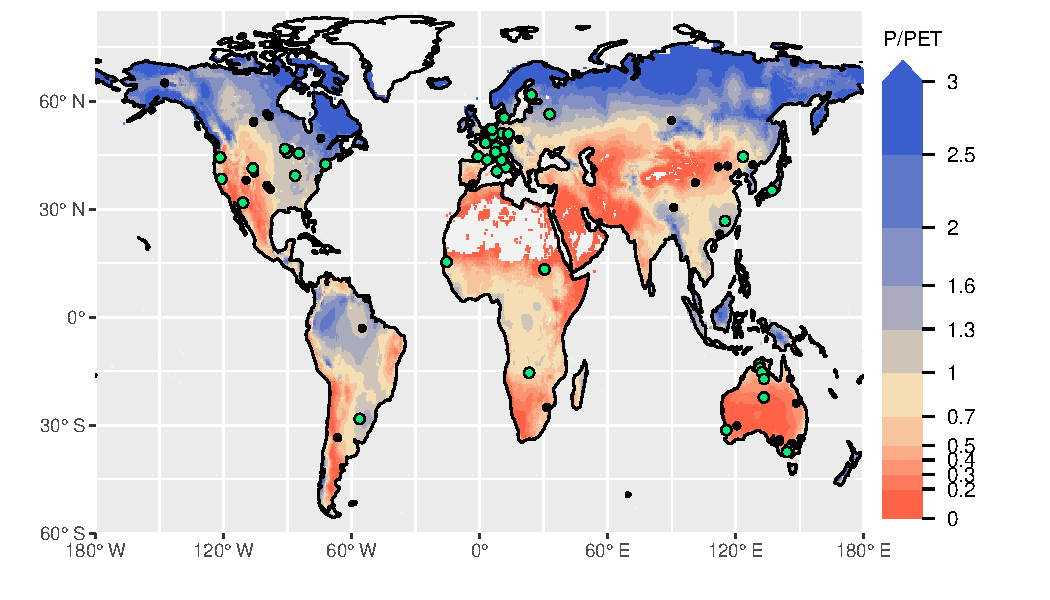
\includegraphics[width=0.8\textwidth]{fig/map_sites.pdf}
    \caption{Overview of sites selected for model calibration (green dots) and evaluation (green and black dots). All sites and additional information are listed in Tab. \ref{tab:sites}. The colour scale represents aridity, quantified as the ratio of precipitation over potential evapotranspiration from \citet{greve14}.}
    \label{fig:map_sites}
\end{figure}

\label{sec:sites}

\subsubsection{Data filtering}
\label{sec:datafiltering}
GPP predictions by the P-model are compared to GPP estimates from the FLUXNET 2015 Tier 1 data set (downloaded on 13 November, 2016). We used GPP based on the nighttime partitioning method \citep{Reichstein2005-mp} (GPP\textunderscore NT\textunderscore VUT\textunderscore REF) and filtered out negative daily GPP values, data for which more than 50\% of the half-hourly data are gap-filled and for which the daytime and nighttime partitioning methods (GPP\textunderscore DT\textunderscore VUT\textunderscore REF and GPP\textunderscore NT\textunderscore VUT\textunderscore REF, respectively) are inconsistent, i.e., the upper and lower 2.5\% quantiles of the difference between GPP values quantified by each method. For additional simulation sets, model calibration and evaluation was performed using GPP data based on the daytime partitioning method (GPP\textunderscore DT\textunderscore VUT\textunderscore REF) \citep{lasslop10} with analogous filtering steps, and GPP data based on an alternative method that fits a constant ecosystem respiration rate as the net ecosystem exchange under conditions where PPFD tends to zero (FULL\textunderscore Ty, \citet{wang17natpl}). For all calibration and evaluation, we removed data points before the ``MODIS era'' (before 18th of February, 2000).

\subsection{Evaluation methods}
\label{sec:methods_eval}

We evaluated both simulated LUE and GPP. The P-model  (Sect. \ref{sec:theory}) predicts variations in LUE across sites (space) and months (monthly LUE $= m'$), while simulated GPP is affected by the PPFD and fAPAR data used as model forcing (Eq. \ref{eq:lue_identification} and Sect. \ref{sec:forcingdata}). Conversely, ``observed'' LUE is calculated as $\text{LUE}_\text{obs} = \text{GPP}_\text{obs} / (\text{fAPAR} \cdot \text{PPFD})$ and the evaluation is thus also affected by the PPFD and fAPAR data. The evaluation of LUE tests the added explanatory power of the P-model compared to models that rely on fixed prescribed LUE values. Evaluating GPP facilitates the comparison of the model performance to similar models of terrestrial GPP. Model performance for GPP is benchmarked against a null model (NULL), which assumes a temporally constant and spatially uniform LUE. The LUE for the NULL model is fitted to observed GPP using splined MODIS FPAR and GPP data from the NT method, see Tab. \ref{tab:setups}. Thus, while LUE is constant, the NULL model preserves the spatial and temporal patterns in APAR ($= \text{fAPAR} \cdot \text{PPFD}$).

\subsubsection{Components of variability}
\label{sec:evalmethod_variability}
For LUE, we separately analysed spatial (mean annual values by site) and monthly means only for the FULL setup. For GPP, we analyzed spatial, annual, seasonal (mean by day-of-year), 8-daily, and the variability in daily anomalies from the mean seasonal cycle for all setups. The seasonal variability was determined for different Koeppen-Geiger climatic zones (see Tab. \ref{tab:kgclimate}). Information about the association of sites with climatic zones was extracted from \citet{falge17}. Evaluations were made only for climatic zones with at least five sites. For each component of variability, we calculated the adjusted coefficient of determination ($R^2_\text{adj}$, thereafter referred to as $R^2$), and the root mean square error (RMSE). Figures showing correlations between simulated and observed values additionally present the mean bias, the slope of the linear regression model, and the number of data points ($N$).

\begin{table}
\caption{Description of Koeppen-Geiger climate zones (based on \citet{falge17}) and number of sites for which data is available per climate zone and hemisphere. Only zones with data from more than three sites are shown.} 
\centering
\begin{tabular}{llll}
  \toprule
  Code & $N$ north & $N$ south & Description \\ 
  \midrule
   Aw   & -- & 5 &  Tropical savannah with dry winter \\ 
   BSk  & 5 & -- & Arid steppe cold \\ 
   Cfa  & 11 & -- & Warm temperate fully humid with hot summer \\ 
   Cfb  & 19 & 5 & Warm temperate fully humid with warm summer \\ 
   Csa  & 12 & -- & Warm temperate with dry and hot summer \\ 
   Csb  & 4 & -- & Warm temperate with dry and warm summer \\ 
   Dfb  & 17 & -- & Cold fully humid warm summer \\ 
   Dfc  & 22 & -- & Cold fully humid cold summer \\ 
%   ET   & 4 & -- & Polar tundra \\ 
   \bottomrule
  \end{tabular}
  \label{tab:kgclimate}
\end{table}


\subsubsection{Drought response}
\label{sec:droughtresponse}
The bias in GPP (modelled minus observed) was calculated for 20 days before and 80 days after the onset of a drought event as identified by \citet{stocker18newphyt} for 36 sites. Drought events (fLUE droughts) are periods of consecutive days where soil moisture, separated from other drivers using neural networks, reduces LUE below a given threshold. The data specifying the timing and duration of drought events was downloaded from \textit{Zenodo} \citep{flue}. We then re-arranged the data to align all drought events at all sites, normalised data to their median value during the ten days before the onset of droughts (normalisation by subtracting median), and computed quantiles per day, where `day' is defined with respect to the onset of each drought event.



\section{Evaluation results}
\label{sec:results}

\subsection{GPP variability across scales}
\label{sec:results_gpp}


Tables \ref{tab:rsq} and \ref{tab:rmse} provide an overview of model performance ($R^2$ and RMSE) in simulating GPP at different scales. The ORG setup captures 69\% of the variance in observed GPP with data aggregated to 8-day means (60’450 data points). Model performance both with respect to explained variance ($R^2$) and the RMSE is improved by including the effects of temperature on quantum yield efficiency in the BRC model setup  ($R^2 = 72$\%), and by including the effects of soil moisture stress in the FULL model setup ($R^2 = 75$\%, Fig. \ref{fig:modobs_xdaily}). Both the BRC and FULL model setup outperform the NULL model.

 % This table is created by eval_pmodel.Rmd, section 'Metrics table'
\begin{table}
\caption{$R^2$ of simulated and observed GPP based on different model setups and for different components of variability.} 
\begin{tabular}{lllllll}
  \toprule
  Setup & 8-daily & Spatial & Annual & Seasonal & var(daily) & var(annual) \\ 
  \midrule
  FULL & 0.75 & 0.70 & 0.70 & 0.74 & 0.28 & 0.09 \\ 
  BRC & 0.72 & 0.66 & 0.62 & 0.73 & 0.26 & 0.06 \\ 
  ORG & 0.69 & 0.62 & 0.57 & 0.69 & 0.25 & 0.06 \\ 
  NULL & 0.69 & 0.64 & 0.58 & 0.71 & 0.25 & 0.04 \\ 
  %NULLpft & 0.71 & 0.66 & 0.61 & 0.73 & 0.25 & 0.03 \\ 
  \midrule
  FULL\_FPARitp & 0.73 & 0.70 & 0.70 & 0.74 & 0.25 & 0.09 \\ 
  FULL\_EVI & 0.70 & 0.56 & 0.47 & 0.72 & 0.29 & 0.14 \\ 
  \midrule
  FULL\_DT & 0.65 & 0.69 & 0.70 & 0.65 & 0.30 & 0.08 \\ 
  FULL\_NTsub & 0.67 & 0.70 & 0.70 & 0.68 & 0.30 & 0.09 \\ 
  FULL\_Ty & 0.69 &  &  & 0.69 & 0.49 & \\ 
  \bottomrule
  \end{tabular}
\label{tab:rsq}
\end{table}

 % This table is created by eval_pmodel.Rmd, section 'Metrics table'
\begin{table}
\caption{Root mean square error (RMSE) of simulated and observed GPP based on different model setups and for different components of variability.} 
\begin{tabular}{lllllll}
  \toprule
  Setup & 8-daily & Spatial & Annual & Seasonal & var(daily) & var(annual) \\ 
  \midrule
  FULL & 1.91 & 421.49 & 396.48 & 1.74 & 1.61 & 149.90 \\ 
  BRC & 2.01 & 455.58 & 444.06 & 1.80 & 1.61 & 151.65 \\ 
  ORG & 2.13 & 485.62 & 474.46 & 1.92 & 1.60 & 152.91 \\ 
  NULL & 2.10 & 468.14 & 478.02 & 1.85 & 1.56 & 153.26 \\ 
  %NULLpft & 2.04 & 452.12 & 461.23 & 1.79 & 1.58 & 154.35 \\ 
  \midrule
  FULL\_FPARitp & 1.98 & 427.46 & 402.94 & 1.77 & 1.71 & 148.96 \\ 
  FULL\_EVI & 2.10 & 523.04 & 535.66 & 1.85 & 1.56 & 143.11 \\ 
  \midrule
  FULL\_DT & 2.08 & 390.45 & 363.55 & 1.94 & 1.73 & 155.03 \\ 
  FULL\_NTsub & 2.05 & 418.65 & 392.20 & 1.90 & 1.73 & 150.76 \\ 
  FULL\_Ty & 1.86 &  &  & 1.75 & 1.37 & \\ 
  \bottomrule
  \end{tabular}
\label{tab:rmse}
\end{table}

\begin{figure}[!ht]
    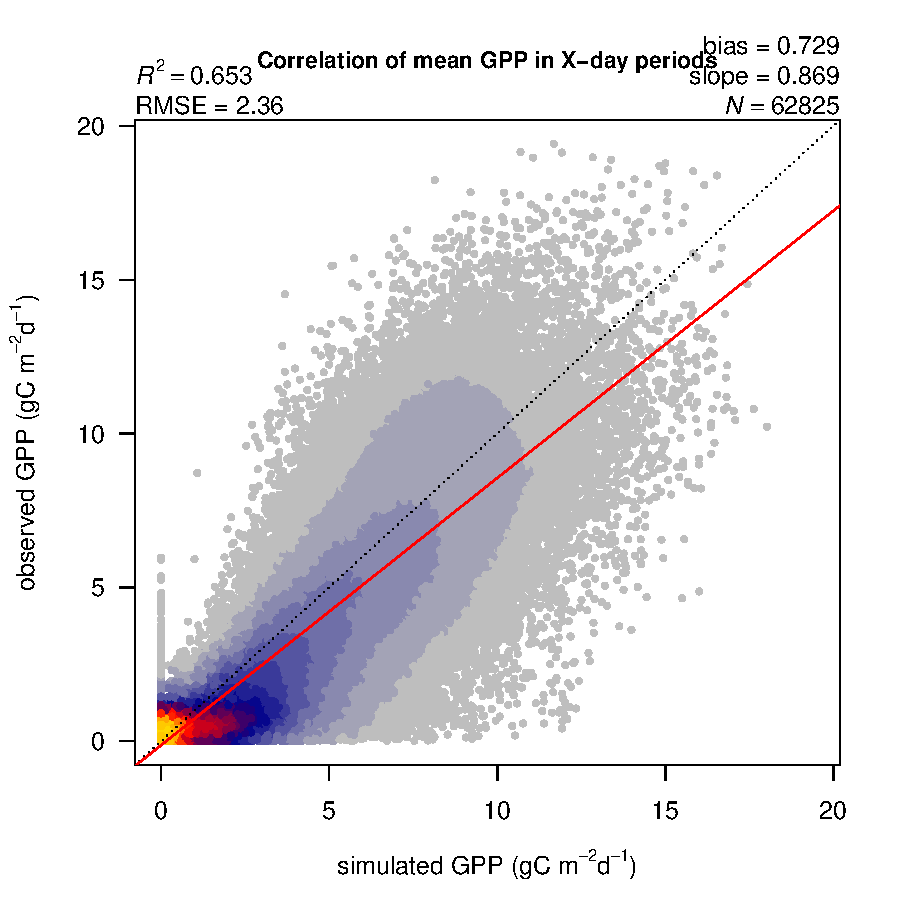
\includegraphics[width=\textwidth]{fig/modobs_xdaily.pdf}
    \caption{Correlation of observed and modelled GPP values of all sites pooled, mean over 8-day periods, for the model setup FULL (a) and NULL (b).}
    \label{fig:modobs_xdaily}
\end{figure}

The \rsq\ for simulated GPP, aggregated to annual totals, ranges from 0.57 (ORG) to 0.70 (FULL). The NULL model achieves an \rsq\ of 0.58. Most of the explanatory power of the different models for predicting annual total GPP stems from their power in predicting between-site (``spatial'') variations (Fig. \ref{fig:modobs_spatialannual}). The \rsq\ for spatial variations ranges from 0.62 (ORG) to 0.70 (FULL), and 0.64 for the NULL model. In contrast, inter-annual  variations at a site are poorly simulated (\rsq : 0.06-0.09 for P-model setups, and 0.04 for the NULL model). Inter-annual variations are generally much smaller than between site variations. Thus, capturing them is challenging. Inter-annual GPP variations are generally better simulated at sites where the variability is high and in particular at dry sites. 

\begin{figure}[!ht]
    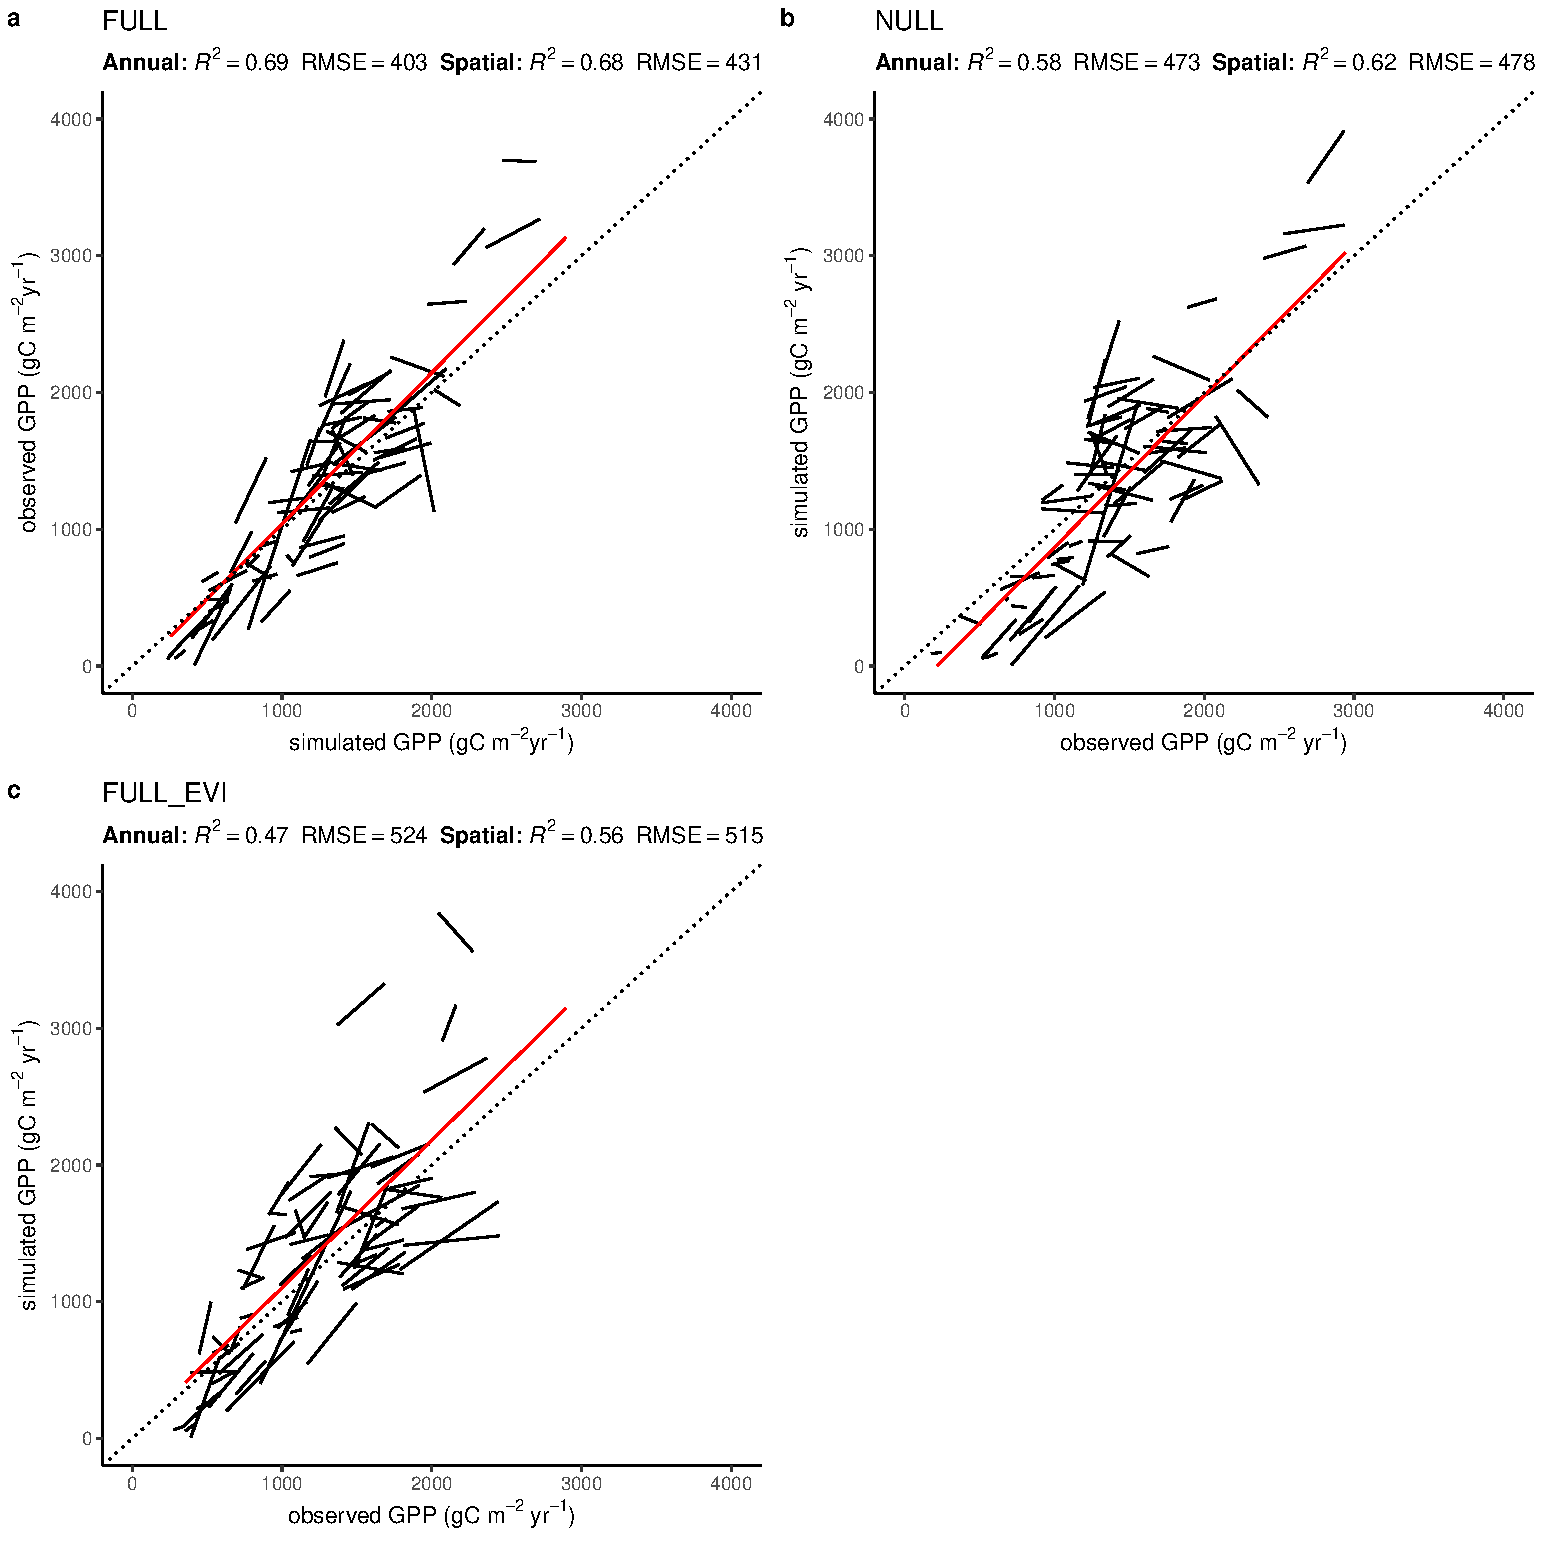
\includegraphics[width=\textwidth]{fig/modobs_spatial_annual.pdf}
    \caption{Correlation of modelled and observed annual GPP in simulations FULL (a), NULL (b) and FULL\textunderscore EVI (c). The red line and text are based on means across years by site and represents spatial (across-site) variations. Black lines and text are based on annual values, one line for each site. Lines represent linear regressions. $R^2$ and RMSE statistics for annual values (black text) are based on pooled data from all sites. For a perfect fit between modelled and observed annual GPP values, all black lines (representing the linear regression model of annual values for a single site) would lie on the 1:1 line and have a slope of 1. Slopes that deviate substantially from 1, or even are negative, for some sites shows poor model performance in capturing inter-annual variability.}
    \label{fig:modobs_spatialannual}
\end{figure}


\subsubsection{Seasonal variations}
\label{sec:results_seasonal}
Seasonal variations are generally reliably simulated (\rsq : 0.69-0.74 for P-model setups, and \rsq : 0.71 for the NULL model, Fig. \ref{fig:season}). Also the NULL model captures most of the seasonal variability, especially in climate zones Dfb and Dfc, and Cfb and Cfa. This indicates that seasonal GPP variations are largely driven by seasonal changes in insolation (PPFD) and vegetetation greenness (fAPAR). Accounting for temperature effects on the quantum yield efficiency reduces the overestimation of GPP in spring, except in the case of climate zone Dfb. Observed GPP increases are lagged compared to vegetation greenness, with a delay of up to 2 months at some sites (e.g., US-Los). This lag is clearly visible at almost all sites in Dfb. The early season high bias is largely absent for sites in climate zone Cfb, where observed GPP starts increasing early and the simulations match the observations except at sites CZ-wet, DE-Hai, and FR-Fon, where the simulated start of season is simulated too early.

GPP is overestimated during the dry season in climate zones with a marked dry season (Aw, BSk, Csa, and Csb) in model setups that do not account for soil moisture stress (ORG, BRC, NULL). The NULL model has the largest bias. High VPD during dry periods reduces simulated LUE and leads to lower GPP values and a smaller bias in all the P-model setups (ORG, BRC, FULL). The empirical soil moisture stress function applied in setup FULL eliminates the dryness-related bias in zones Aw, Csa, and Csb and substantially reduces this bias for sites in zone BSk. Observations suggest that GPP declines to values around zero during dry periods at sites in zone BSk (mostly savannah vegetation and grasslands, see Table \ref{tab:sites}). The remaining bias in the FULL model, which includes the soil moisture stress function, is related to the fact that fAPAR remains relatively high and that the soil moisture stress function does not decline to zero.

The ORG and BRC models tend to underestimate peak season GPP more strongly compared to the FULL model. This is a direct consequence of the calibration which balances errors across all data points. Across-site average peak-season maximum GPP is accurately captured by the FULL model in all zones (Fig. \ref{fig:season}), except for an underestimation of GPP in zones Aw and Cfb, and an overestimation in zone Csa. Site-level evaluations suggests no clear relationship between peak-season underestimation and vegetation type in zone Cfb. The overestimation of peak-season GPP in zone Csa is caused by a high bias at sites with evergreen broadleaved vegetation (FR-Pue, IT-Cp2, IT-Cpz); sites with other vegetation types show no consistent peak season bias. 

 \begin{figure}[!ht]
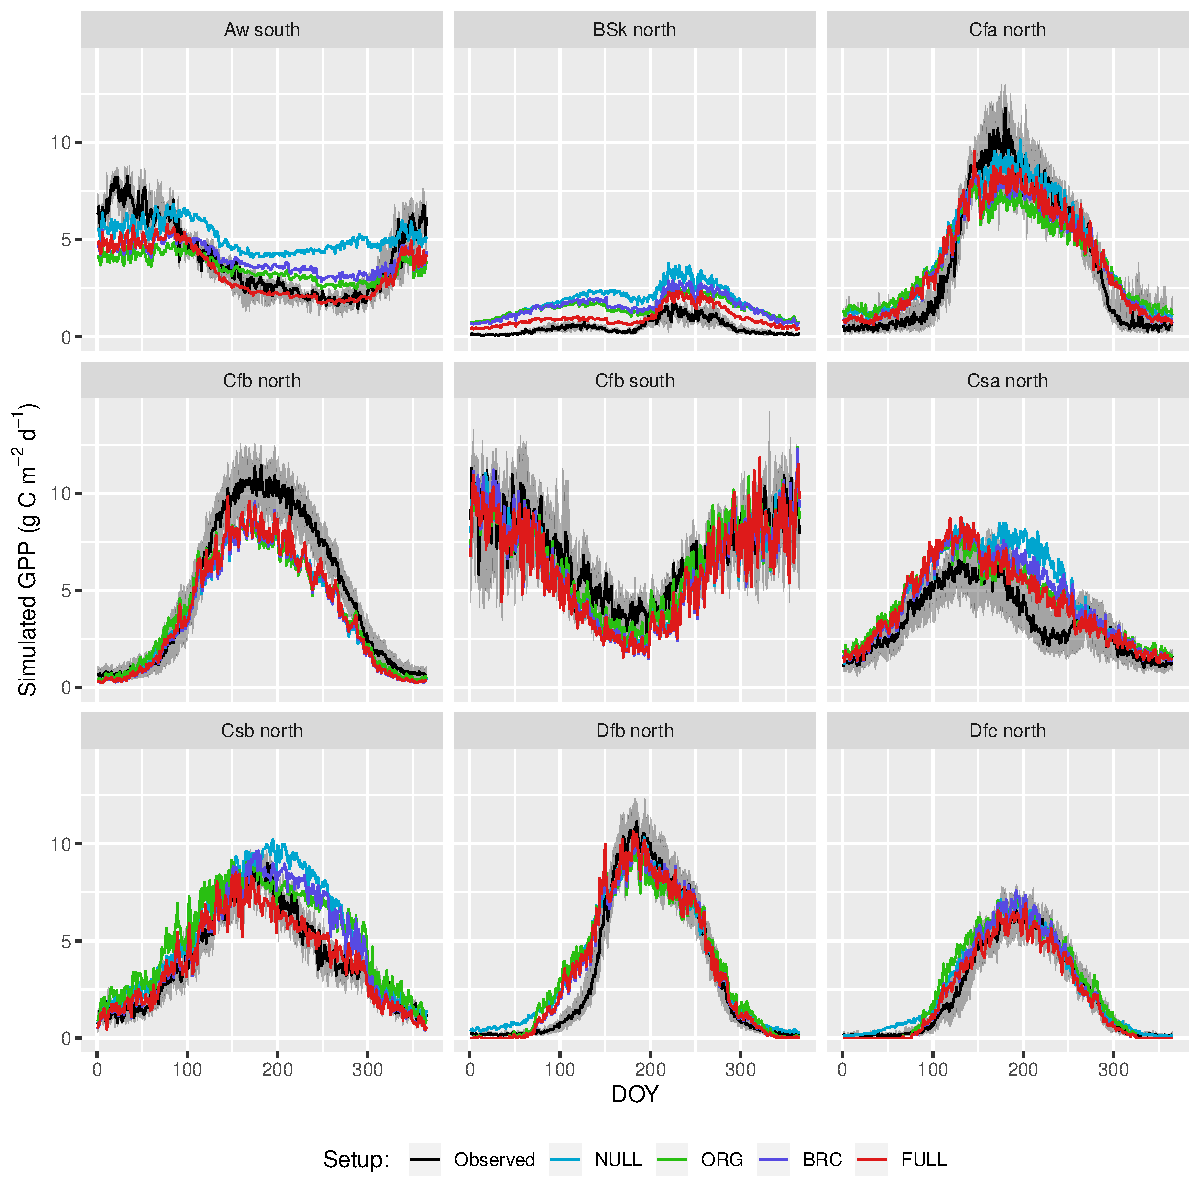
\includegraphics[width=\textwidth]{fig/meandoy_byzone.pdf}
\caption{Mean seasonal cycle. Observations are given by the black line and grey band, representing the median and 33/66 \% quantiles of all data (multiple sites and years) pooled by climate zone. Coloured lines represent different model setups. The annotation above each plot specifies the climate zone (see Tab. \ref{tab:kgclimate}). Only climate zones are shown here for which data from at least five sites was available.}
    \label{fig:season}
\end{figure}


\subsection{Drought response}
\label{sec:results_droughtresponse}

The P-model setups that do not include the soil moisture stress function (ORG and BRC) systematically overestimate GPP during droughts (Fig. \ref{fig:modobs_droughtresponse}). This bias increases sharply at the onset of drought events and continues to increase throughout the drought period. The bias is strongly reduced by applying the empiricial soil moisture stress function (Eq. \ref{eq:soilmstress}) in the FULL model. A small bias remains also in the FULL model. This stems from overestimated values at a few sites (in particular AU−DaP, US-Cop, US-SRG, US-SRM, US-Var, US-Whs, US-Wkg), mostly grasslands and sites in seasonally dry climate zones (Aw, BSk, and Csa, see Fig. \ref{fig:season}), where flux measurements indicate an almost complete shut-down of photosynthetic activity during the dry season. In contrast, the fAPAR data (MODIS FPAR) suggest values substantially greater than zero at these sites during these periods. This suggests either contributions to PAR absorption by photosynthetically inactive tissue, underestimation of LUE sensitivity to dry soils at these sites, or an overestimation of the rooting zone moisture availability by SPLASH.

\begin{figure}[!ht]
    \centering
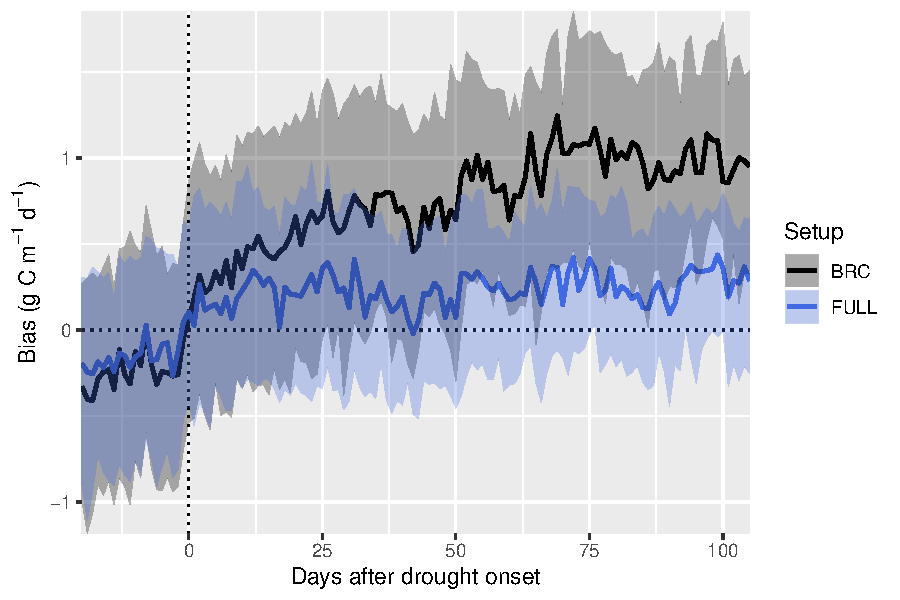
\includegraphics[width=0.5\textwidth]{fig/droughtresponse.pdf}
    \caption{Bias in simulated GPP during the course of drought events. Simulated GPP is from a simulation with (FULL) and without (BRC) accounting for soil moisture stress. The timing of drought events is taken from \citet{stocker18newphyt} and is identified by an apparent soil moisture-related reduction of observed light use efficiency at 36 FLUXNET sites. The bias is calculated as simulated minus observed GPP. Data from multiple drought events and sites are aligned by the date of drought onset and aggregated across all sites and events (lines for medians, shaded ranges from the 33\% and 66\% quantiles).}
    \label{fig:modobs_droughtresponse}
\end{figure}


\subsection{Uncertainty from fAPAR input data}
\label{sec:results_greenness}

Tests of the sensitivity of model performance to alternative fAPAR forcing datasets show that the difference between splined and linearly-interpolated MODI FPAR is negligible. However, model performance is generally better using MODIS FPAR compared to simulations using MODIS EVI. Spatial variations are well captured using MODIS FPAR (Fig. \ref{fig:modobs_spatialannual}, \rsq : 0.70) compared to MODIS EVI (\rsq : 0.56). However, the \rsq\ of inter-annual variations is 0.14 for MODIS EVI and 0.09 for MODIS FPAR. In terms of biases in climate zones, the overestimation of GPP during the dry period in zone BSk is larger when using MODIS EVI than when using MODIS FPAR (Fig. \ref{fig:season_greenness}, right). The positive spring bias in simulated GPP in zone Dfb is present irrespective of the source of the fAPAR forcing (Fig. \ref{fig:season_greenness}, left), as is the peak-season bias of GPP in zones BSk, Cfb, and Csb. Differences between the EVI and FPAR-forced simulations depend on vegetation type. The EVI-forced simulation tends to be low biased in evergreen needle-leaved vegetation, and has generally lower values in all evergreen vegetation types compared to the FPAR-forced simulation. However, there is no general difference in model bias between simulations made with the two forcings in other vegetation types. 

 \begin{figure}[!ht]
    \centering
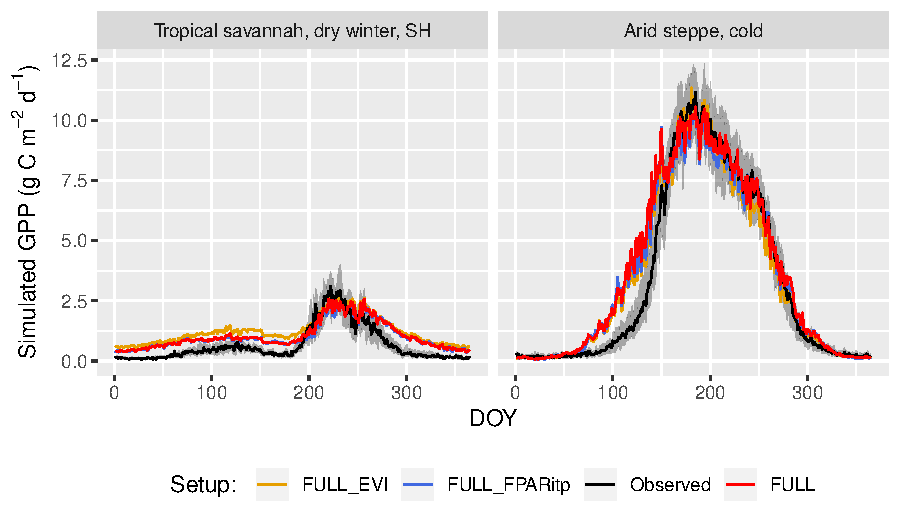
\includegraphics[width=0.8\textwidth]{fig/meandoy_byzone_greenness.pdf}
    \caption{Mean seasonal cycle for model setups with different greenness forcing data. Observations are given by the black line and grey band, representing the median and 33/66 \% quantiles by day-of-year (DOY) of all data (multiple sites and years) pooled by climate zone. Coloured lines represent model setups, forced with different greenness data. The annotation above each plot specifies the climate zone (see Tab. \ref{tab:kgclimate}). Climate zones shown here are illustrative examples.}
    \label{fig:season_greenness}
\end{figure}


\subsection{Uncertainty from GPP target data}
\label{sec:results_gppdata}

Model predictions compare better to GPP data based on the Ty than either the DT or NT methods. For GPP,  8-day means, the model achieves an \rsq\ of 0.69 when compared to GPP Ty (model setup FULL\textunderscore Ty), compared to 0.65 and 0.67 for the DT and NT methods, respectively (FULL\textunderscore DT and FULL\textunderscore NTsub, Tab. \ref{tab:rsq}, Fig. \ref{fig:modobs_10d_gppdata}). Variations in daily GPP anomalies are much better captured in evaluations with Ty (\rsq : 0.49) than DT or NT (\rsq : 0.30). Spatial and annual correlations were not evaluated for Ty because of missing data. The systematic low bias of simulated peak-season GPP in climatic zone Cfb is not affected by the choice of GPP evaluation data (Fig. \ref{fig:modobs_10d_gppdata}).

The systematic differences in the level of model-data agreement depending on the target GPP dataset (Fig. \ref{fig:modobs_10d_gppdata}) reflect the fact that these datasets are derived using decomposition methods with different sensitivity to diurnal changes in temperature.

 \begin{figure}[!ht]
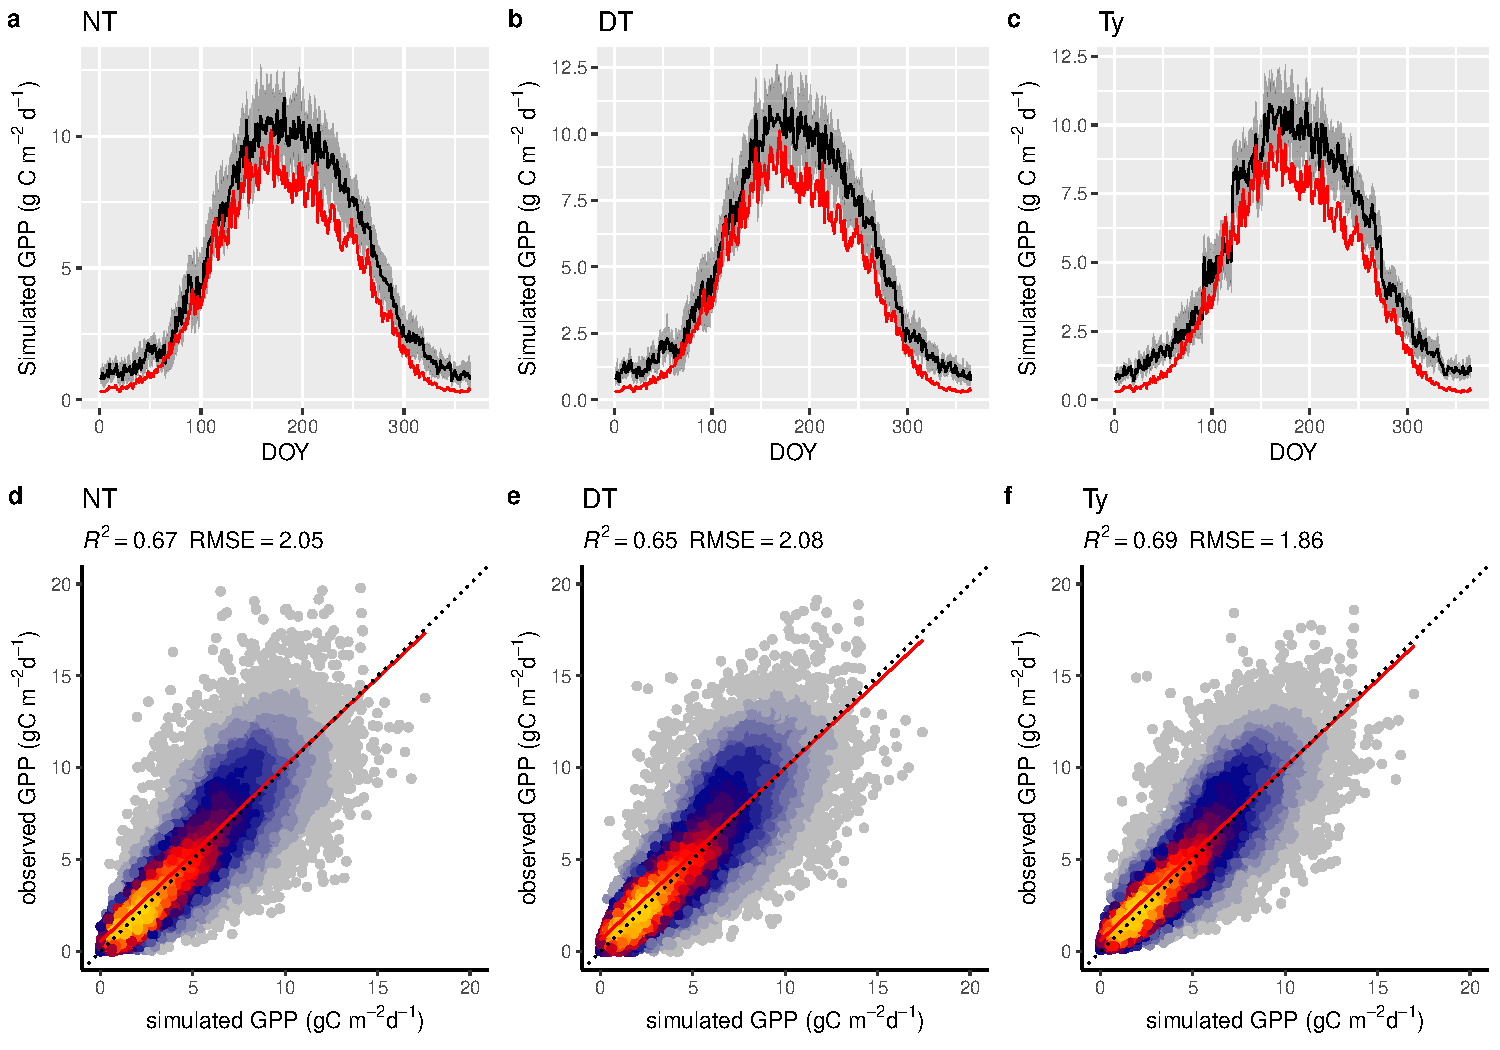
\includegraphics[width=\textwidth]{fig/meandoy_modobs_gpp_data.pdf}
    \caption{Model performance subject to comparison with different flux decomposition methods for GPP. (a-c): Mean seasonal cycle of simulated (red) and observed GPP (black) based on different flux decomposition methods. The grey band represents the 33/66 \% quantiles of observed GPP by day-of-year (DOY). (d-f): Correlation of observed and simulated GPP values of all sites pooled, mean over 8-day periods. `Observed GPP' refers to the different flux decomposition methods: DT for the daytime method (setup FULL\textunderscore DT), NT for the nighttime method (setup FULL\textunderscore NTsub) and Ty (setup FULL\textunderscore Ty) for the method applied for data used in \citet{wang17rs}. Dotted lines in (d-f) represent the 1:1 relationship, red lines represent the fitted linear regressions.}
    \label{fig:modobs_10d_gppdata}
\end{figure}


\subsection{LUE}
\label{sec:results_lue}
The FULL version of the P-model captures 37\% of the variability in mean annual LUE across all sites and across the full range of observed mean annual LUE values and vegetation types (Fig. \ref{fig:lue}). 53 \% of the observed LUE variation within vegetation types is captured by the model through the relationships with climate, without the need to specify parameters for specific vegetation types. 

33\% of the variability in monthly mean LUE is captured by the model, with data from all sites and years pooled (Fig. \ref{fig:lue}). The model overestimates monthly LUE values and underestimates LUE at the lowest and highest end of the LUE range respectively. The low-end overestimation is reflected by the overestimation of GPP in the spring at winter-cold sites (Sect. \ref{sec:results_seasonal}) and during soil moisture droughts (Sect. \ref{sec:results_droughtresponse}). The underestimation of high monthly values is not clearly linked to any particular vegetation type.

 \begin{figure}[!ht]
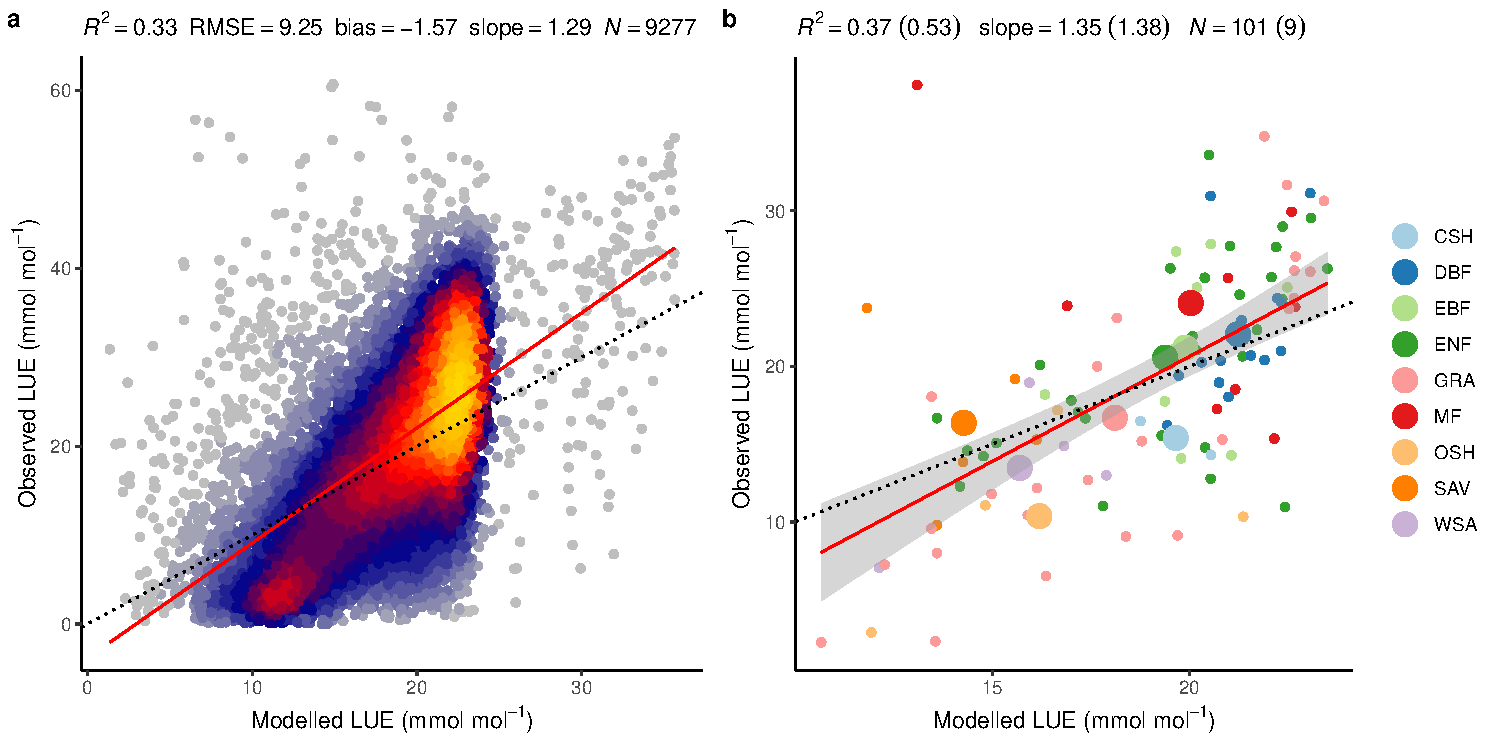
\includegraphics[width=\textwidth]{fig/modobs_lue.pdf}
    \caption{Modelled (simulations FULL) versus observed LUE. (a) Mean monthly LUE with data pooled from all sites and available years. (b) Mean annual LUE by site (small dots and color) and vegetation type (large dots and color). Model performance metrics are given at the top with numbers in brackets referring to the regression of data aggregated by vegetation types and non-bracketed numbers for data aggregated by sites. Dotted lines represent the 1:1 relationship, red lines represent the fitted linear regression to all data in (a) and to mean annual LUE by site in (b). The grey band in (b) represents the 95 \% confidence interval of the linear regression. Vegetation types are: closed shrubland (CSH); deciduous broadleaf forest (DBF); evergreen broadleaf forest (EBF); evergreen needleleaf forest (ENF); grassland (GRA); mixed deciduous and evergreen needleleaf forest (MF); open shrubland (OSH); savanna ecosystem (SAV); woody savanna (WSA). }
    \label{fig:lue}
\end{figure}



% \subsubsection{VPD}

% Vapour pressure deficit ($D$) is calculated from vapour pressure (CRU) or specific humidity (WATCH-WFDEI) input data. In general, $D$ is the difference between actual and saturation vapour pressure:
% \begin{equation}
%     D = e_a - e_s
% \end{equation}
% We calculate saturation vapour pressure ($e_s$, in Pa) following Allen et al. (2005) as a function of temperature  as
% \begin{equation}
% e_s = 611 \; \exp \left( {\frac{17.27\;T_C}{T_C+237.3}} \right)
% \end{equation}
% $T_C$ is the temperature expressed in units of degrees Celsius. Note that Allen et al. (2005) use 6.108 instead of 6.11. The Python implementation uses daily maximum and daily minimum temperature, which is equivalent to above formulation with $T=(T_{\text{min}}+T_{\text{max}})/2$. $e_a$ is provided by CRU as an input dataset. WATCH-WFDEI provides specific humidity data ($q$), which can be converted to the mass mixing ratio of water vapor to dry air ($w$) (dimensionless) by
% \begin{equation}
%     w = \frac{q}{1-q}
% \end{equation}
% and finally to actual vapour pressure by
% \begin{equation}
%     e_a = P \frac{w R_v}{R_d + w R_v}
% \end{equation}
% where $P$ is the atmospheric pressure (Pa), $R_v$ is the specific gas constant for water vapour and $R_d$ is the specific gas constant for dry air. The specific gas constants are calculated from the universal gas constant $R$ and the molecular mass $M$ as $R_{\text{specific}}=R/M$. ($R$ is 8.3143 J mol$^{-1}$ K$^{-1}$. The molecular mass of dry air is $M_d=$ 28.963 g mol$^{-1}$ and the molecular mass of water vapor is $M_v=$ 18.02 g mol$^{-1}$.) Atmospheric pressure is assumed to be at standard conditions (101325 Pa) corrected for local elevation (barometric formula adopted from SPLASH, Eq. 20 in Davis et al., 2017).




% \begin{table}
% \centering
% \begin{tabular}{ p{1.2cm} p{2.5cm} p{2.5cm} p{4cm} l }
% \multicolumn{5}{l}{\textbf{ WATCH-WFDEI }} \\
% \hline
% \textbf{symbol} & \textbf{variable name} & \textbf{file name} & \textbf{variable description} & \textbf{units} \\
% \hline
% $T$ & \texttt{Tair} & \texttt{Tair\_WFDEI} & 2 m instantaneous air temperature & K \\
% $P_{\text{rain}}$    & \texttt{Rainf}  & \texttt{Rainf\_WFDEI\_CRU} & Rainfall rate, bias corrected with CRU TS3.101 data (TS3.21 for 2010-2012) and gauge ``catch corrected'' (average over previous 3 hrs) & kg m$^{-2}$ s$^{-1}$ \\  
% $P_{\text{snow}}$    & \texttt{Snowf} & \texttt{Snowf\_WFDEI\_CRU} & Snowfall rate, bias corrected with CRU TS3.101 data (TS3.21 for 2010-2012) and gauge ``catch corrected'' (average over previous 3 hrs)  & kg m$^{-2}$ s$^{-1}$ \\  
% $R_{\text{SW}}$    & \texttt{SWdown} & \texttt{SWdown\_WFDEI} & Short-wave downwards surface radiation flux (average over previous 3 hours) & W m$^{-2}$ \\  
% $q$    & \texttt{Qair} & \texttt{Qair\_WFDEI} & 2 m instantaneous specific humidity & kg kg$^{-1}$ \\  
% $p$    & \texttt{PSurf} & \texttt{PSurf\_WFDEI} & Instantaneous surface pressure & Pa \\ 
% \hline
% \end{tabular}
% \caption{Variables used from WATCH-WFDEI meteorological data.}
% \label{tab:meteovars}
% \end{table}

\section{Discussion}
\label{sec:discussion}

The performance of the P-model can be compared to results obtained from other remote-sensing driven GPP models (RS-models). In its FULL setup, the P-model achieves an \rsq\ of 0.75 and a RMSE of 1.91 g C m$^{-2}$ d$^{-1}$, in simulating 8-day mean GPP and evaluated against GPP data (NT method) from 131 sites. This can be compared to predictions from the VPM model (\rsq : 0.74, RMSE: 2.08 g C m$^{-2}$ d$^{-1}$, 113 sites, 8-daily, \citet{Zhang2017-yr}), or BESS (\rsq : 0.67, RMSE: 2.58 g C m$^{-2}$ d$^{-1}$, 113 sites, 8-daily, \citet{jiang16rse}). The performance of the P-model in simulating \textit{annual} GPP across all 131 sites (\rsq : 0.70) can be compared to results from MODIS GPP (MOD17A2, \rsq = 0.73, 12 sites, \citet{heinsch06}, and for the updated version MOD17A2H: \rsq = 0.62, 18 sites, \citet{wang17rs}). 

The coefficients of determination (\rsq ) of simulated versus observed values are lower for LUE (0.37 for the spatial correlation in the FULL setup, Fig. \ref{fig:lue}b) than for GPP (0.70 for the spatial correlation in the FULL setup). This is because GPP variations are strongly driven by variations in absorbed light (PPFD$\cdot$fAPAR), which are observed and used for modelling. In contrast, variations in LUE cannot be observed directly. Using remotely-sensed information for estimating LUE variations, e.g., based on sun-induced fluorescence \citep{frankenberg18, li18gcb, ryu19rse} or alternative reflectance indices \citep{gamon92, gamon16pnas, Badgley2017-tw}, is an active field of research and the separation of remotely sensed signals into contributions by LUE and absorbed light remains challenging \citep{porcarcastell14, ryu19rse}. Other remote sensing-based GPP models rely on vegetation type-specific model parameters for LUE \citep{Zhang2017-yr, running04, jiang16rse}. The P-model in its FULL setup explains 53\% of the variations in LUE across sites aggregated to vegetation types without relying on vegetation or biome-type specific parametrisations. In its ORG setup, it explains 21\% of the variations (not shown), and 51\% of the variations when excluding sites classified as `open shrublands', which tend have a substantially lower LUE than simulated by the P-model (not shown). In spite of this substantial portion of explained variability, the NULL model with its temporally constant and spatially uniform LUE achieves higher \rsq\ values for GPP than the ORG P-model setup at the spatial, annual, and seasonal scales (Tab. \ref{tab:rsq}). This indicates that the spatial and temporal variations in absorbed light are the main drivers of GPP in LUE-type models and underlines the importance of evaluation against a NULL model benchmark. Taken together, these findings demonstrate that the P-model offers a simple but powerful method for simulating terrestrial GPP using readily available input datasets and a very small number of free (calibratable) parameters. Here, three parameters are calibrated (for the FULL setup). Other model parameters are derived from independent field and laboratory measurements.

% It appears surprising, however, that the NULL model achieves only a slightly lower \rsq\ (0.64, spatial) compared to the FULL model (0.70, spatial), while using a constant and uniform LUE across all sites and time. 

Accounting for the temperature-dependence of the quantum yield efficiency ($\varphi_0$) clearly improves model predictions. The parameter $\varphi_0$ is commonly treated as a constant in global vegetation models \citep{rogers17}. Our results indicate potential for improving DVM photosynthesis routines by accounting for the temperature-dependence of $\varphi_0$. 

$\varphi_0$ appears as a linear scalar in the LUE model. However, the magnitude of this scalar is uncertain and depends on whether incomplete light absorption by the leaf is included in the definition of $\varphi_0$ or in fAPAR data. We have used MODIS FPAR and MODIS EVI data to define fAPAR in different model setups.  While the two are well correlated, their absolute values differ. Hence, we have calibrated an \textit{apparent} quantum yield efficiency ($\widehat{\varphi_0}$) to GPP data separately for different fAPAR datasets, thereby implicitly distinguishing what components of light absorption factors are contained in the fAPAR data. The leaf absorbtance $a_L$, which is typically taken to be around 0.8 in global vegetation models \citep{rogers17} is similar to the ratio of fitted $\widehat{\varphi_0}$ values for simulation FULL and FULL\textunderscore EVI, here calculated as 0.67 (Tab. \ref{tab:setups}).

An improvement in model performance is obtained by accounting for soil moisture stress using an empirical function.  However, the use of an empirical function masks underlying processes. Furthermore, the use of an empirical function is not consistent with the optimality approach that underlies the P-model. The reduced bias using an empirical soil moisture stress function implies something is missing in the theoretical approach which rests on an assumed constancy of the unit costs of transpiration ($a$ in Eq. \ref{eq:optimality_chi}). \citet{prentice14ecollett} provide a definition of $a$ that is explicit in terms of plant hydraulic traits and physical properties that determine water transport along the plant-soil-atmosphere continuum. In particular, $a \propto ( \Delta \Psi k_s )^{-1}$, where $\Delta \Psi$ is the maximum daytime difference in leaf-to-soil water potential and $k_s$ is the sapwood area-specific permeability. However, large variations in stomatal conductance are known to occur in response to relatively fast soil dry-downs (time scale of days) \citep{keenan10agrformet, egea11, stocker18newphyt}. This suggests the potential to improve the P-model by allowing the unit cost of transpiration to be a function of rooting-zone moisture availability, and by coupling stomatal conductance with the soil water balance.

Observational uncertainty could affect both parameter calibration and model evaluation. \citet{keenan19natee} found a systematic bias in GPP estimates based on the nighttime partitioning method due to inhibition of leaf respiration in the light \citep{kok49, wehr16}, which affects fluxes unevenly throughout the season and across vegetation types. However, we found no clear difference in model-data agreement, nor in fitted parameters,  in comparisons of three alternative GPP datasets that use different approaches to decompose net \coo\ exchange fluxes from eddy covariance measurements into ecosystem respiration and GPP terms.

We have found a consistent early-season high-bias in simulated GPP for numerous sites in regions with deciduous broadleaved vegetation in temperate and cold climates (in particular US-MMS, IT-Col, US-WCr, US-UMd, US-UMB, and US-Ha1), and also in mixed and needle-leaved stands (in particular US-Syv, US-NR1, FI-Hyy, CA-Qfo, and CA-Man). Additional analyses (not shown) suggested that this bias is not related to soil temperatures or the difference between soil and air temperatures in spring. The P-model, as applied here, uses daily air temperature for simulating acclimation. Hence, a bias is to be expected in view of the known delay in the resumption of photosynthesis after a cold dormant period \citep{huner93, oquist03, adams04, verhoeven14, bowling18}. Such delays are mediated by a biochemical downregulation of photosynthesis, not included in the P-model, i.a. using xanthophyll carotenoids for photoprotection \citep{adams04} to balance photochemical and biochemical processes -- the former being less steeply temperature-dependent \citep{oquist03}. Cold-acclimation is a strategy to cope with frozen sap transport vessels during periods when air temperature is already high \citep{bowling18}, or for protecting against frost damage during early season cold spells \citep{vitasse14}. Approaches accounting for a delayed resumption of photosynthesis after cold periods \citep{pelkonen80, bergh98, makela04} offer scope for further improvement of the P-model.

There is a positive bias in simulated GPP during the dry season at a number of sites where the vegetation phenology is influenced by drought. The positive bias is related to the combination of using prescribed fAPAR data, which shows substantial absorption by non-green vegetation, and insufficient sensitivity of simulated LUE to soil drying. However, GPP is accurately simulated at other sites affected by seasonally recurring water stress. The modelled sensitivity to dry soils is determined by the soil moisture stress function, which depends on the mean aridity of the site as estimated using a fixed depth soil moisture "bucket". Accounting for variability in rooting zone depth, which may also be influenced by local topographical factors and access to groundwater \citep{fan13sci, fan17pnas} may help to minimise model biases in drought-prone areas.

The current implementation of the P-model involves some simplifications in terms of climate drivers by using average daily meteorological conditions, measured above the canopy, as input. Optimality in balancing carbon and water costs for average daily conditions is not necessarily equivalent to optimality in balancing integrated water and carbon costs over the diurnal cycle. Large variations in ambient conditions over a diurnal cycle, combined with a non-linear dependence of costs on these conditions suggest that the approach of taking average daily conditions may be an over-simplification. Nevertheless, prior evaluations have shown robust and accurate predictions of optimal $\chi$ across a range conditions \citep{wang17natpl}. Using above-canopy VPD values instead of VPD at the leaf surface for scaling water losses implicitly assumes a perfectly coupled atmospheric boundary layer. Using above-canopy air temperature instead of leaf temperatures introduces a bias when the two become decoupled \citep{michaletz15tee}. The impact of these simplifications may be minor but should be evaluated. %Furthermore, the light use efficiency model, using prescribed fAPAR, implies that no distinction is made between light absorptance by the canopy of diffuse and direct radiation. 

A further simplification is that investment in electron transport capacity (expressed by \jmax ) and investments in the carboxylation capacity (expressed by \vcmax ) are coordinated so that for conditions with which the model is forced (here, monthly means of daily averages), photosynthesis operates at the co-limitation point of the light- and Rubisco-limited assimilation rates and an effective linear relationship between absorbed light and mean assimilation emerges. This assumption follows from the \textit{coordination hypothesis} \citep{chen93, haxeltine96}, which itself can be understood as an optimality principle \citep{haxeltine96}, and is well supported by observations \citep{maire12po}. However, this coordination is contingent on the time scale at which photosynthetic acclimation occurs, which is not known precisely  \citep{smithdukes13gcb, way14}. By simulating $\chi$ usingh monthly mean meteorological variables, we assume a monthly time scale of acclimation. This is probably a conservative estimate \citep{smithdukes17, veres84}. Considering the concave relationship of assimilation rates and absorbed light that follows from the FvCB model for a given \jmax , linearly scaling a given monthly LUE term with daily varying absorbed light levels should lead to an overestimation of assimilation rates at high light levels. This overestimation should disappear as the time scale over which light levels are averaged is increased. However, our results do not confirm these expectations. The fact that the model did not exhibit a systematic error in simulating GPP variations when applied at the daily time scale suggests that the day-to-day variability in light levels is relatively small compared to the within-day variability.

\begin{figure}[!ht]
    \centering
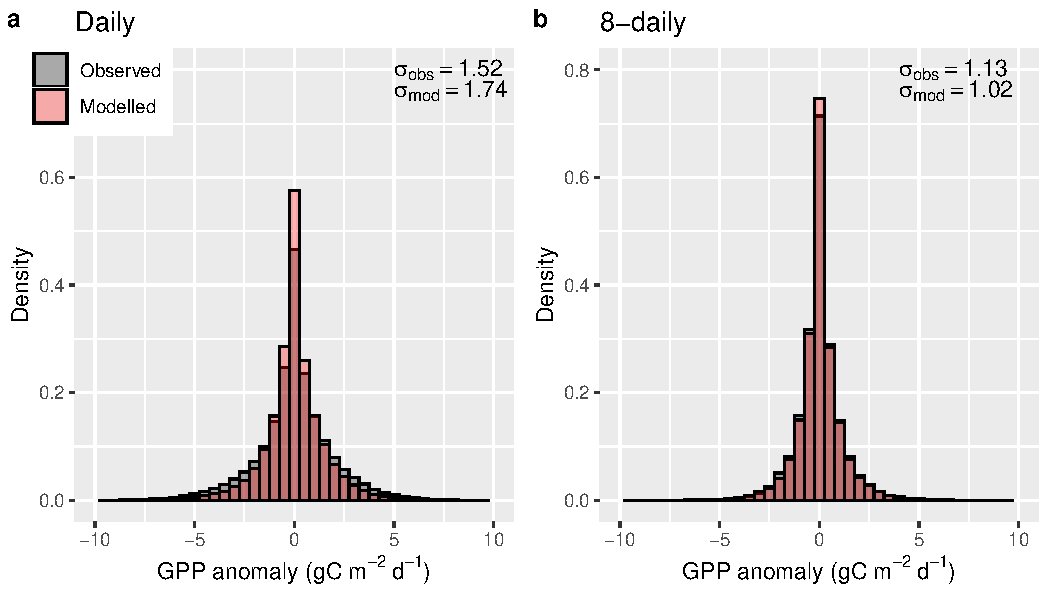
\includegraphics[width=0.7\textwidth]{fig/hist_anomalies.pdf}
    \caption{Distribution of anomalies from the mean seasonal cycle, evaluated for daily values (a) and 8-day means (b).} 
    \label{fig:modobs_anomalies}
\end{figure}


\section{Conclusion}

The P-model provides a simple, parameter-sparse but powerful method to predict photosynthetic capacity and light use efficiency across a wide range of climatic conditions and vegetation types. It provides a basis for a terrestrial light use efficiency model driven by remotely sensed vegetation greenness. Using optimality principles for the formulation of the P-model reduces its dependence on uncertain or vegetation type-specific parameters and enables robust predictions of GPP and its variations through the seasons, between years, and across space. Further work is required to develop a distinct treatment of C$_4$ vegetation for global applications and additional evaluations are needed to examine the P-model's sensitivity to increasing \coo . We have shown that accounting for the effects of low soil moisture and the reduction in the quantum yield efficiency under low temperatures improves model performance. There is potential to include below-ground water limitation effects in the mechanistic optimality framework of the P-model. 


\clearpage

\section{Acknowledgements}


\section{Data and code availability}

The P-model is implemented as an R package (\textit{rpmodel}) and available through \url{https://stineb.github.io/rpmodel/}. Model outputs (daily) are available on Zenodo XXX. Code for all evaluations presented here is available through \url{https://github.com/stineb/eval_pmodel}. 

\section{Appendix}

% This table is created by 
\begin{longtable}{lllllllll}
  \toprule
Site & Lon. & Lat. & Period & Veg. & Clim. & N & Calib. & Reference \\ 
  \midrule
  AR-SLu & -66.46 & -33.46 & 2009-2011 & MF & Bwk & 446 &  & \citet{AR-SLu} \\ 
  AR-Vir & -56.19 & -28.24 & 2009-2012 & ENF & Csb & 749 & Y & \citet{AR-Vir} \\ 
  AT-Neu & 11.32 & 47.12 & 2002-2012 & GRA & Dfc & 3243 &  & \citet{AT-Neu} \\ 
  AU-Ade & 131.12 & -13.08 & 2007-2009 & WSA & Aw & 532 & Y & \citet{AU-Ade} \\ 
  AU-ASM & 133.25 & -22.28 & 2010-2013 & ENF & BSh & 1045 & Y & \citet{AU-ASM} \\ 
  AU-Cpr & 140.59 & -34.00 & 2010-2014 & SAV & BSk & 1370 &  & \citet{AU-Cpr} \\ 
  AU-Cum & 150.72 & -33.61 & 2012-2014 & EBF & Cfa & 744 &  & \citet{AU-Cum} \\ 
  AU-DaP & 131.32 & -14.06 & 2007-2013 & GRA & Aw & 1402 & Y & \citet{AU-DaP} \\ 
  AU-DaS & 131.39 & -14.16 & 2008-2014 & SAV & Aw & 2265 & Y & \citet{AU-DaS} \\ 
  AU-Dry & 132.37 & -15.26 & 2008-2014 & SAV & Aw & 1598 & Y & \citet{AU-Dry} \\ 
  AU-Emr & 148.47 & -23.86 & 2011-2013 & GRA & Bwk & 755 &  & \citet{AU-Emr} \\ 
  AU-Fog & 131.31 & -12.55 & 2006-2008 & WET & Aw & 878 & Y & \citet{AU-Fog} \\ 
  AU-Gin & 115.71 & -31.38 & 2011-2014 & WSA & Csa & 942 & Y & \citet{AU-Gin} \\ 
  AU-GWW & 120.65 & -30.19 & 2013-2014 & SAV & Bwk & 663 &  & \citet{AU-GWW} \\ 
  AU-Lox & 140.66 & -34.47 & 2008-2009 & DBF & Bsh & 273 &  & \citet{AU-Lox} \\ 
  AU-RDF & 132.48 & -14.56 & 2011-2013 & WSA & Bwh & 431 &  & \citet{AU-RDF} \\ 
  AU-Rig & 145.58 & -36.65 & 2011-2014 & GRA & Cfb & 1130 &  & \citet{AU-Rig} \\ 
  AU-Rob & 145.63 & -17.12 & 2014-2014 & EBF & Csb & 337 &  & \citet{AU-Rob} \\ 
  AU-Stp & 133.35 & -17.15 & 2008-2014 & GRA & BSh & 1318 & Y & \citet{AU-Stp} \\ 
  AU-TTE & 133.64 & -22.29 & 2012-2013 & OSH & BWh &  94 &  & \citet{AU-TTE} \\ 
  AU-Tum & 148.15 & -35.66 & 2001-2014 & EBF & Cfb & 4335 &  & \citet{AU-Tum} \\ 
  AU-Wac & 145.19 & -37.43 & 2005-2008 & EBF & Cfb & 979 &  & \citet{AU-Wac} \\ 
  AU-Whr & 145.03 & -36.67 & 2011-2014 & EBF & Cfb & 1065 & Y & \citet{AU-Whr} \\ 
  AU-Wom & 144.09 & -37.42 & 2010-2012 & EBF & Cfb & 934 & Y & \citet{AU-Wom} \\ 
  AU-Ync & 146.29 & -34.99 & 2012-2014 & GRA & BSk & 392 &  & \citet{AU-Ync} \\ 
  BE-Bra & 4.52 & 51.31 & 1996-2014 & MF & Cfb & 4208 & Y & \citet{BE-Bra} \\ 
  BE-Vie & 6.00 & 50.31 & 1996-2014 & MF & Cfb & 4733 & Y & \citet{BE-Vie} \\ 
  BR-Sa3 & -54.97 & -3.02 & 2000-2004 & EBF & Am & 1206 &  & \citet{BR-Sa3} \\ 
  CA-Man & -98.48 & 55.88 & 1994-2008 & ENF & Dfc & 1411 &  & \citet{CA-Man} \\ 
  CA-NS1 & -98.48 & 55.88 & 2001-2005 & ENF & Dfc & 771 &  & \citet{CA-NS1} \\ 
  CA-NS2 & -98.52 & 55.91 & 2001-2005 & ENF & Dfc & 873 &  & \citet{CA-NS2} \\ 
  CA-NS3 & -98.38 & 55.91 & 2001-2005 & ENF & Dfc & 1069 &  & \citet{CA-NS3} \\ 
  CA-NS4 & -98.38 & 55.91 & 2002-2005 & ENF & Dfc & 610 &  & \citet{CA-NS4} \\ 
  CA-NS5 & -98.48 & 55.86 & 2001-2005 & ENF & Dfc & 912 &  & \citet{CA-NS5} \\ 
  CA-NS6 & -98.96 & 55.92 & 2001-2005 & OSH & Dfc & 913 &  & \citet{CA-NS6} \\ 
  CA-NS7 & -99.95 & 56.64 & 2002-2005 & OSH & Dfc & 709 &  & \citet{CA-NS7} \\ 
  CA-Qfo & -74.34 & 49.69 & 2003-2010 & ENF & Dfc & 1812 &  & \citet{CA-Qfo} \\ 
  CA-SF1 & -105.82 & 54.48 & 2003-2006 & ENF & Dfc & 525 &  & \citet{CA-SF1} \\ 
  CA-SF2 & -105.88 & 54.25 & 2001-2005 & ENF & Dfc & 675 &  & \citet{CA-SF2} \\ 
  CA-SF3 & -106.01 & 54.09 & 2001-2006 & OSH & Dfc & 651 &  & \citet{CA-SF3} \\ 
  CH-Cha & 8.41 & 47.21 & 2005-2014 & GRA & Cfb & 2885 &  & \citet{CH-Cha} \\ 
  CH-Dav & 9.86 & 46.82 & 1997-2014 & ENF & ET & 4444 &  & \citet{CH-Dav} \\ 
  CH-Fru & 8.54 & 47.12 & 2005-2014 & GRA & Cfb & 2566 & Y & \citet{CH-Fru} \\ 
  CH-Lae & 8.37 & 47.48 & 2004-2014 & MF & Cfb & 3204 & Y & \citet{CH-Lae} \\ 
  CH-Oe1 & 7.73 & 47.29 & 2002-2008 & GRA & Cfb & 2104 & Y & \citet{CH-Oe1} \\ 
  CN-Cha & 128.10 & 42.40 & 2003-2005 & MF & Dwb & 982 &  & \citet{CN-Cha} \\ 
  CN-Cng & 123.51 & 44.59 & 2007-2010 & GRA & Bsh & 1113 & Y & \citet{CN-Cng} \\ 
  CN-Dan & 91.07 & 30.50 & 2004-2005 & GRA & ET & 647 &  & \citet{CN-Dan} \\ 
  CN-Din & 112.54 & 23.17 & 2003-2005 & EBF & Cfa & 917 &  & \citet{CN-Din} \\ 
  CN-Du2 & 116.28 & 42.05 & 2006-2008 & GRA & Dwb & 616 &  & \citet{CN-Du2} \\ 
  CN-Ha2 & 101.33 & 37.61 & 2003-2005 & WET & ET & 1030 &  & \citet{CN-Ha2} \\ 
  CN-HaM & 101.18 & 37.37 & 2002-2004 & GRA &  & 688 &  & \citet{CN-HaM} \\ 
  CN-Qia & 115.06 & 26.74 & 2003-2005 & ENF & Cfa & 992 & Y & \citet{CN-Qia} \\ 
  CN-Sw2 & 111.90 & 41.79 & 2010-2012 & GRA & Bsh & 237 &  & \citet{CN-Sw2} \\ 
  CZ-BK1 & 18.54 & 49.50 & 2004-2008 & ENF & Dfb & 1100 &  & \citet{CZ-BK1} \\ 
  CZ-BK2 & 18.54 & 49.49 & 2004-2006 & GRA & Dfb & 161 &  & \citet{CZ-BK2} \\ 
  CZ-wet & 14.77 & 49.02 & 2006-2014 & WET & Cfb & 2605 & Y & \citet{CZ-wet} \\ 
  DE-Gri & 13.51 & 50.95 & 2004-2014 & GRA & Cfb & 3387 & Y & \citet{DE-Gri} \\ 
  DE-Hai & 10.45 & 51.08 & 2000-2012 & DBF & Cfb & 3435 & Y & \citet{DE-Hai} \\ 
  DE-Lkb & 13.30 & 49.10 & 2009-2013 & ENF & Cfb & 1001 &  & \citet{DE-Lkb} \\ 
  DE-Obe & 13.72 & 50.78 & 2008-2014 & ENF & Cfb & 2043 & Y & \citet{DE-Obe} \\ 
  DE-RuR & 6.30 & 50.62 & 2011-2014 & GRA & Cfb & 1195 & Y & \citet{DE-RuR} \\ 
  DE-SfN & 11.33 & 47.81 & 2012-2014 & WET & Cfb & 750 &  & \citet{DE-SfN} \\ 
  DE-Spw & 14.03 & 51.89 & 2010-2014 & WET & Cfb & 1339 & Y & \citet{DE-Spw} \\ 
  DE-Tha & 13.57 & 50.96 & 1996-2014 & ENF & Cfb & 4887 & Y & \citet{DE-Tha} \\ 
  DK-NuF & -51.39 & 64.13 & 2008-2014 & WET & ET & 882 & Y & \citet{DK-NuF} \\ 
  DK-Sor & 11.64 & 55.49 & 1996-2014 & DBF & Cfb & 4483 & Y & \citet{DK-Sor} \\ 
  DK-ZaF & -20.55 & 74.48 & 2008-2011 & WET & ET & 381 &  & \citet{DK-ZaF} \\ 
  DK-ZaH & -20.55 & 74.47 & 2000-2014 & GRA & ET & 1696 &  & \citet{DK-ZaH} \\ 
  ES-LgS & -2.97 & 37.10 & 2007-2009 & OSH & Csa & 794 &  & \citet{ES-LgS} \\ 
  ES-Ln2 & -3.48 & 36.97 & 2009-2009 & OSH & Csa &  69 &  & \citet{ES-Ln2} \\ 
  FI-Hyy & 24.30 & 61.85 & 1996-2014 & ENF & Dfc & 4222 & Y & \citet{FI-Hyy} \\ 
  FI-Lom & 24.21 & 68.00 & 2007-2009 & WET & Dfc & 575 &  & \citet{FI-Lom} \\ 
  FI-Sod & 26.64 & 67.36 & 2001-2014 & ENF & Dfc & 2816 & Y & \citet{FI-Sod} \\ 
  FR-Fon & 2.78 & 48.48 & 2005-2014 & DBF & Cfb & 2827 & Y & \citet{FR-Fon} \\ 
  FR-LBr & -0.77 & 44.72 & 1996-2008 & ENF & Cfb & 2800 & Y & \citet{FR-LBr} \\ 
  FR-Pue & 3.60 & 43.74 & 2000-2014 & EBF & Csa & 4723 & Y & \citet{FR-Pue} \\ 
  GF-Guy & -52.92 & 5.28 & 2004-2014 & EBF & Af & 3719 &  & \citet{GF-Guy} \\ 
  IT-CA1 & 12.03 & 42.38 & 2011-2014 & DBF & Csa & 1036 &  & \citet{IT-CA1} \\ 
  IT-CA3 & 12.02 & 42.38 & 2011-2014 & DBF & Csa & 913 &  & \citet{IT-CA3} \\ 
  IT-Col & 13.59 & 41.85 & 1996-2014 & DBF & Cfa & 2822 & Y & \citet{IT-Col} \\ 
  IT-Cp2 & 12.36 & 41.70 & 2012-2014 & EBF & Csa & 764 & Y & \citet{IT-Cp2} \\ 
  IT-Cpz & 12.38 & 41.71 & 1997-2009 & EBF & Csa & 2601 & Y & \citet{IT-Cpz} \\ 
  IT-Isp & 8.63 & 45.81 & 2013-2014 & DBF & Cfb & 588 & Y & \citet{IT-Isp} \\ 
  IT-Lav & 11.28 & 45.96 & 2003-2014 & ENF & Cfb & 3919 & Y & \citet{IT-Lav} \\ 
  IT-MBo & 11.05 & 46.01 & 2003-2013 & GRA & Dfb & 3236 & Y & \citet{IT-MBo} \\ 
  IT-Noe & 8.15 & 40.61 & 2004-2014 & CSH & Cwb & 3083 & Y & \citet{IT-Noe} \\ 
  IT-PT1 & 9.06 & 45.20 & 2002-2004 & DBF & Cfa & 828 & Y & \citet{IT-PT1} \\ 
  IT-Ren & 11.43 & 46.59 & 1998-2013 & ENF & Dfc & 3043 & Y & \citet{IT-Ren} \\ 
  IT-Ro2 & 11.92 & 42.39 & 2002-2012 & DBF & Csa & 2671 &  & \citet{IT-Ro2} \\ 
  IT-SR2 & 10.29 & 43.73 & 2013-2014 & ENF & Csa & 668 & Y & \citet{IT-SR2} \\ 
  IT-SRo & 10.28 & 43.73 & 1999-2012 & ENF & Csa & 3791 & Y & \citet{IT-SRo} \\ 
  IT-Tor & 7.58 & 45.84 & 2008-2014 & GRA & Dfc & 1487 & Y & \citet{IT-Tor} \\ 
  JP-MBF & 142.32 & 44.39 & 2003-2005 & DBF & Dfb & 471 &  & \citet{JP-MBF} \\ 
  JP-SMF & 137.08 & 35.26 & 2002-2006 & MF & Cfa & 1288 & Y & \citet{JP-SMF} \\ 
  NL-Hor & 5.07 & 52.24 & 2004-2011 & GRA & Cfb & 2131 & Y & \citet{NL-Hor} \\ 
  NL-Loo & 5.74 & 52.17 & 1996-2013 & ENF & Cfb & 4507 & Y & \citet{NL-Loo} \\ 
  NO-Adv & 15.92 & 78.19 & 2011-2014 & WET & ET & 151 &  & \citet{NO-Adv} \\ 
  NO-Blv & 11.83 & 78.92 & 2008-2009 & SNO & ET & 112 &  & \citet{NO-Blv} \\ 
  RU-Che & 161.34 & 68.61 & 2002-2005 & WET & Dfc & 313 &  & \citet{RU-Che} \\ 
  RU-Cok & 147.49 & 70.83 & 2003-2014 & OSH & Dfc & 985 &  & \citet{RU-Cok} \\ 
  RU-Fyo & 32.92 & 56.46 & 1998-2014 & ENF & Dfb & 4042 & Y & \citet{RU-Fyo} \\ 
  RU-Ha1 & 90.00 & 54.73 & 2002-2004 & GRA & Dfc & 519 &  & \citet{RU-Ha1} \\ 
  SD-Dem & 30.48 & 13.28 & 2005-2009 & SAV & BWh & 762 & Y & \citet{SD-Dem} \\ 
  SN-Dhr & -15.43 & 15.40 & 2010-2013 & SAV & BWh & 686 & Y & \citet{SN-Dhr} \\ 
  US-AR1 & -99.42 & 36.43 & 2009-2012 & GRA & Cfa & 1011 &  & \citet{US-AR1} \\ 
  US-AR2 & -99.60 & 36.64 & 2009-2012 & GRA & Cfa & 882 &  & \citet{US-AR2} \\ 
  US-ARb & -98.04 & 35.55 & 2005-2006 & GRA & Cfa & 414 &  & \citet{US-ARb} \\ 
  US-ARc & -98.04 & 35.55 & 2005-2006 & GRA & Cfa & 488 &  & \citet{US-ARc} \\ 
  US-Blo & -120.63 & 38.90 & 1997-2007 & ENF & Csb & 1827 &  & \citet{US-Blo} \\ 
  US-Cop & -109.39 & 38.09 & 2001-2007 & GRA & BSk & 1067 &  & \citet{US-Cop} \\ 
  US-GBT & -106.24 & 41.37 & 1999-2006 & ENF & Dfc & 541 &  & \citet{US-GBT} \\ 
  US-GLE & -106.24 & 41.37 & 2004-2014 & ENF & Dfb & 2254 & Y & \citet{US-GLE} \\ 
  US-Ha1 & -72.17 & 42.54 & 1991-2012 & DBF & Dfb & 3259 & Y & \citet{US-Ha1} \\ 
  US-KS2 & -80.67 & 28.61 & 2003-2006 & CSH & Cfa & 1263 &  & \citet{US-KS2} \\ 
  US-Los & -89.98 & 46.08 & 2000-2014 & WET & Dfb & 2071 & Y & \citet{US-Los} \\ 
  US-Me1 & -121.50 & 44.58 & 2004-2005 & ENF & Csb & 287 &  & \citet{US-Me1} \\ 
  US-Me2 & -121.56 & 44.45 & 2002-2014 & ENF & Csb & 3525 & Y & \citet{US-Me2} \\ 
  US-Me6 & -121.61 & 44.32 & 2010-2014 & ENF & Csb & 1283 &  & \citet{US-Me6} \\ 
  US-MMS & -86.41 & 39.32 & 1999-2014 & DBF & Cfa & 3524 & Y & \citet{US-MMS} \\ 
  US-Myb & -121.77 & 38.05 & 2010-2014 & WET & Csb & 1153 &  & \citet{US-Myb} \\ 
  US-NR1 & -105.55 & 40.03 & 1998-2014 & ENF & Dfc & 4084 &  & \citet{US-NR1} \\ 
  US-PFa & -90.27 & 45.95 & 1995-2014 & MF & Dfb & 3679 &  & \citet{US-PFa} \\ 
  US-Prr & -147.49 & 65.12 & 2010-2013 & ENF & Dfc & 546 &  & \citet{US-Prr} \\ 
  US-SRG & -110.83 & 31.79 & 2008-2014 & GRA & BSk & 2146 & Y & \citet{US-SRG} \\ 
  US-SRM & -110.87 & 31.82 & 2004-2014 & WSA & BSk & 3093 & Y & \citet{US-SRM} \\ 
  US-Syv & -89.35 & 46.24 & 2001-2014 & MF & Dfb & 2045 & Y & \citet{US-Syv} \\ 
  US-Ton & -120.97 & 38.43 & 2001-2014 & WSA & Csa & 4321 & Y & \citet{US-Ton} \\ 
  US-Tw1 & -121.65 & 38.11 & 2012-2014 & WET & Csa & 688 &  & \citet{US-Tw1} \\ 
  US-Tw4 & -121.64 & 38.10 & 2013-2014 & WET & Csa & 325 &  & \citet{US-Tw4} \\ 
  US-UMB & -84.71 & 45.56 & 2000-2014 & DBF & Dfb & 4015 & Y & \citet{US-UMB} \\ 
  US-UMd & -84.70 & 45.56 & 2007-2014 & DBF & Dfb & 2050 & Y & \citet{US-UMd} \\ 
  US-Var & -120.95 & 38.41 & 2000-2014 & GRA & Csa & 2981 & Y & \citet{US-Var} \\ 
  US-WCr & -90.08 & 45.81 & 1999-2014 & DBF & Dfb & 2333 & Y & \citet{US-WCr} \\ 
  US-Whs & -110.05 & 31.74 & 2007-2014 & OSH & BSk & 1561 &  & \citet{US-Whs} \\ 
  US-Wi0 & -91.08 & 46.62 & 2002-2002 & ENF & Dfb & 228 &  & \citet{US-Wi0} \\ 
  US-Wi3 & -91.10 & 46.63 & 2002-2004 & DBF & Dfb & 415 &  & \citet{US-Wi3} \\ 
  US-Wi4 & -91.17 & 46.74 & 2002-2005 & ENF & Dfb & 712 & Y & \citet{US-Wi4} \\ 
  US-Wi6 & -91.30 & 46.62 & 2002-2003 & OSH & Dfb & 351 &  & \citet{US-Wi6} \\ 
  US-Wi9 & -91.08 & 46.62 & 2004-2005 & ENF & Dfb & 302 &  & \citet{US-Wi9} \\ 
  US-Wkg & -109.94 & 31.74 & 2004-2014 & GRA & BSk & 2676 &  & \citet{US-Wkg} \\ 
  ZA-Kru & 31.50 & -25.02 & 2000-2010 & SAV & BSh & 2124 &  & \citet{ZA-Kru} \\ 
  ZM-Mon & 23.25 & -15.44 & 2000-2009 & DBF & Aw & 641 & Y & \citet{ZM-Mon} \\ 
  \bottomrule
\caption{Sites used for evaluation. Lon. is longitude, negative values indicate west longitude; Lat. is latitude, positive values indicate north latitude; Veg. is vegetation type: deciduous broadleaf forest (DBF); evergreen broadleaf forest (EBF); evergreen needleleaf forest (ENF); grassland (GRA); mixed deciduous and evergreen needleleaf forest (MF); savanna ecosystem (SAV); shrub ecosystem (SHR); wetland (WET).} 
\label{tab:sites}
\end{longtable}


%% \\\\\\\\\\\\\\\\\\\\\\\\\\\\\\\\\\\\\\\\\\\\\\\\\\\\\\\
%% PHOTORESPIRATORY COMPENSATION POINT
%% ///////////////////////////////////////////////////////
\subsection{Photorespiratory Compensation Point $\Gamma^\ast$}
\label{sec:gammastar}
The temperature and pressure-dependent photorespiratory compensation point in absence of dark respiration $\Gamma^\ast(T,p)$ is calculated from its value at standard temperature ($T_0=$ 25${^\circ}$C) and atmospheric pressure ($p_0 = $101325 Pa), referred to as $\Gamma^\ast_{25, p_0}$. It is modified by temperature following an Arrhenius-type temperature response function $f_{\text{Arrh}}(T_K, \Delta H_{\Gamma\ast})$ with activation energy $\Delta H_{\Gamma\ast}$, and is corrected for atmospheric pressure $p(z)$ at elevation $z$. 
\begin{equation}
\label{eq:gammastar}
    \Gamma^\ast (T_K, z) = \Gamma^\ast_{25, p_0} \; f_{\text{Arrh}}(T_K, \Delta H_{\Gamma\ast}) \; \frac{p(z)}{p_0}
\end{equation}
Values of $\Delta H_{\Gamma\ast}$ and $\Gamma^\ast_{25, p_0}$ are taken from \citet{bernacchi01}. The latter is converted to Pa and standardised to $p_0$ simply by multiplication with $p_0$ ($\Gamma^\ast_{25, p_0} = 42.75\; \mu$mol mol$^{-1} \cdot 10^{-6} \cdot 101325$ Pa $ = 4.332$ Pa). $\Delta H_{\Gamma\ast}$ is 37830 J mol$^{-1}$. All parameter values are summarised in Tab. \ref{tab:params}. The function $p(z)$ is defined in Sec \ref{sec:press}. Note that $T_K$ indicates that the respective temperature value is given in Kelvin and $T_{K,0}=$ 298.15 K.

To correct for effects by temperature following the Arrhenius Equation with its form $x(T_K)=\exp(c-\Delta H_a/(T_K R))$, the temperature-correction function $f_{\text{Arrh}}(T_K, \Delta H_a)$, used in Eq. \ref{eq:gammastar} and further equations below, is given by:
\begin{equation}
    f_{\text{Arrh}}(T_K) = x(T_K)/x(T_{K,0}) = \exp \left( \frac{\Delta H (T_K - T_{K,0})}{T_{K,0}\: R\: T_K} \right) 
\end{equation}
where $\Delta H$ is the respective activation energy (e.g., $\Delta H_{\Gamma\ast}$ in Eq. \ref{eq:gammastar}), and $R$ is the universal gas constant (8.3145 J mol$^{-1}$ K$^{-1}$).

\subsubsection{Deriving $\Gamma^\ast$}
The temperature and pressure dependency of $\Gamma^\ast$ follows from the temperature dependencies of $K_c$, $K_o$, $V_\text{c,max}$, and $V_\text{o,max}$ and the pressure dependency of $pO_2(p)$:
\begin{equation}
\label{eq:gsbasic}
    \Gamma^\ast (T_K, p) = \frac{pO_2(p)\: K_c(T_K)\: V_\text{omax}(T_K)}
                        {2\: K_o(T_K)\: V_\text{cmax}(T_K)}
\end{equation}
$pO_2(p)$ is the partial pressure of atmospheric oxygen (Pa) and scales linearly with $p(z)$. $K_c$ is the Michaelis-Menten constant for carboxylation (Pa); $K_o$ is the Michaelis-Menten constant for oxygenation (Pa); $V_\text{cmax}$ is maximum rate of carboxylation ($\mu$mol~m$^{-2}$~s$^{-1}$); and $V_\text{omax}$ is the maximum rate of oxygenation ($\mu$mol~m$^{-2}$~s$^{-1}$). The temperature-dependency equations for these four terms are given in Table 1 of \citet{bernacchi01} with respective scaling constants $c$ and activation energies $\Delta H_a$ as :
\begin{subequations}
\begin{align}
    K_c(T_K) &= \exp(38.05-79.43/(T_K R)) \\
    K_o(T_K) &= 1000 \cdot \exp(20.30-36.38/(T_K R)) \\
    V_\text{o,max}(T_K) &= \exp(22.98-60.11/(T_K R)) \\
    V_\text{c,max}(T_K) &= \exp(26.35-65.33/(T_K R))
\end{align}
\end{subequations}
By substituting the temperature-dependency equations for each term in Eq. \ref{eq:gsbasic} and rearranging terms, $\Gamma^\ast$ can be written as
\begin{equation}
    \label{eq:gsto}
    \Gamma^\ast(T_K, z) = pO_2(z)\: \exp(6.779-37.83/(T_K R))\;.
\end{equation}
With $pO_2(p)$ at standard atmospheric pressure (101325 Pa) taken to be 21000 Pa, and assuming a constant mixing ratio across the troposphere, its pressure dependence can be expressed as 
\begin{equation}
    \label{eq:oxy}
    pO_2(p) = 0.2095 \cdot p(z)\;
\end{equation}
hence
\begin{equation}
    \label{eq:gstop}
    \Gamma^\ast(T_K, p) = p(z) \exp(5.205-37.83/(T_K R))  % 6.779+\log(0.207254)=5.20519 
\end{equation}
We can use this to calculate $\Gamma^\ast$ at standard temperature ($T_K=$ 298.15 K) and pressure ($p(z)=$ 101325 Pa) as $\Gamma^\ast_{25, p_0} = 4.332$ Pa. 

Note that to convert Eq. \ref{eq:gsto} to the form corresponding to the one given by \citet{bernacchi01}, the partial pressure of oxygen ($pO_2$) has to be assumed at standard conditions. $pO_2$ is approximately 21000 Pa and with the standard atmospheric pressure of 101325 Pa, $pO_2$ can be converted from Pascals to parts-per-million (ppm) as $21000/101325 \times 10^6 = 207254$ ppm = $\exp(12.24)$ ppm. This can be combined with the exponent in Eq. \ref{eq:gsto} to $\exp(12.24) \cdot \exp(6.779) = \exp(19.02)$. This corresponds to the parameter values determining the temperature dependence of $\Gamma^\ast$ given by \citet{bernacchi01} as  $\Gamma^\ast = \exp(19.02-37.83/(T_K R))$.


% FULL DERIVATION WITH STEPS
% , results in the following expression:
% \begin{equation}
%     \Gamma^\ast = \frac{O}{2}\frac{\exp(38.05-79.43/(T_K R))}{1000 \exp(20.30-36.38/(T_K R))}\frac{\exp(22.98-60.11/(T_K R))}{\exp(26.35-65.33/(T_K R))}
% \end{equation}

% \noindent By separating each of the exponents based on the rule of addition returns the following:

% \begin{equation}
%     \Gamma^\ast = \frac{O}{2}\frac{\exp(38.05)\: \exp(-79.43/(T_K R))}{1000 \exp(20.30) \exp(-36.38/(T_K R))}\frac{\exp(22.98) \exp(-60.11/(T_K R))}{\exp(26.35) \exp(-65.33/(T_K R))}
% \end{equation}

% \noindent Sorting the terms based on their temperature-dependence and, using the rule of addition again, combining like terms yields the following:

% \begin{equation}
%     \Gamma^\ast = \frac{O}{2}\frac{\exp(61.03)}{1000 \exp(46.65)}\frac{\exp(101.71/(T_K R))}{\exp(139.54/(T_K R))}
% \end{equation}

% \noindent By using the rule of negative exponents and the rule of addition, the expression may be further simplified as follows:

% \begin{equation}
%     \Gamma^\ast = \frac{O}{2}\frac{\exp(14.38)}{1000}\exp(-37.83/(T_K R))
% \end{equation}

% \noindent Combining the two denominators returns a value of 2000. 
% Note that $\exp(\ln(2000)) = 2000$ and that $\ln(2000) = 7.601$, such that:

% \begin{equation}
%     \Gamma^\ast = O\frac{\exp(14.38)}{\exp(7.601)}\exp(-37.83/(T_K R))
% \end{equation}

% \noindent and when simplified returns the following:

% \begin{equation}
%     \label{eq:gsto}
%     \Gamma^\ast = O\: \exp(6.779-37.83/(T_K R))
% \end{equation}


%% \\\\\\\\\\\\\\\\\\\\\\\\\\\\\\\\\\\\\\\\\\\\\\\\\\\\\\\
%% MICHAELIS-MENTON COEFFICIENT xxxbeni
%% ///////////////////////////////////////////////////////
\subsection{Michaelis-Menten Coefficient of Photosynthesis}
\label{sec:kmm}
The effective Michaelis-Menten coefficient $K$ (Pa) of Rubisco-limited photosynthesis (Eq. \ref{eq:ac}) is determined by the Michaelis-Menten constants for the carboxylation and oxygenation reactions \citep{farquhar80}:
%% ------------------------------------------------------------------------ %%
%% eq:michaelis | Michaelis Menten coefficient
%% ------------------------------------------------------------------------ %%
\begin{equation}
\label{eq:michaelis}
  K(T_K, p) = K_c(T_K)\: \left( 1 + \frac{pO_2(p)}{K_o(T_K)} \right) \;,
\end{equation}
where $K_c$ is the Michaelis-Menten constant for CO$_2$ (Pa), $K_o$ is the Michaelis-Menten constant for the carboxylation and oxygenation reaction, respectively, and $pO_2$ is the partial pressure of oxygen (Pa). $K_c$ and $K_o$ follow a temperature dependence, given by the Arrhenius equation analogously to the temperature dependence of $\Gamma^\ast$ (Eq. \ref{eq:gammastar}):
%% ------------------------------------------------------------------------ %%
%% eq:kcko | Michaelis Menten Kc & Ko coefficients
%% ------------------------------------------------------------------------ %%
\begin{subequations}
\label{eq:kcko}
\begin{align}
  K_c(T_K)& = K_{c25}\: f_{\text{Arrh}}(T_K, \Delta H_{Kc}) \label{eq:kc} \\
    K_o(T_K)& = K_{o25}\: f_{\text{Arrh}}(T_K, \Delta H_{Ko}) \label{eq:ko}
\end{align}
\end{subequations}
Values $\Delta H_{Kc} = 79430$ J mol$^{-1}$, $\Delta H_{Ko} = 36380$ J mol$^{-1}$, $K_{c25} = 39.97$ Pa, and $K_{o25} = 27480$ Pa are taken from \citet{bernacchi01} and (see also Tab. \ref{tab:params}). The latter two have been converted from $\mu$mol mol$^{-1}$ in \citet{bernacchi01} to units of Pa by multiplication with the standard atmosphere (101325 Pa). Note that $K_{c25}$ and $K_{o25}$ are rate constants and are independent of atmospheric pressure. Pressure-dependence of $K$ is solely in $pO_2(p)$ (see Eq. \ref{eq:oxy}).

% where $K_{c25}$ is the Michaelis-Menten constant for CO$_2$ at 25~$^{\circ}$C (Pa), $K_{o25}$ is the Michaelis-Menten constant for O$_2$ at 25~$^{\circ}$C (Pa), $\Delta H_{a,c}$ is the activation energy for carboxylation [79$\,$430 J mol$^{-1}$], $\Delta H_{a,o}$ is the activation energy for oxygenation [36$\,$380 J mol$^{-1}$], $R$ is the universal gas constant [8.31447 J mol$^{-1}$ K$^{-1}$], and $T_K$ is the leaf temperature [K].

% \noindent Once again, leaf temperature, as in Eqns. \ref{eq:michaelis} and \ref{eq:kcko}, may be substituted by the ambient air temperature, $T_{air}$, converted to units of Kelvin. 

% The partial pressure values of $K_{c25}$ and $K_{o25}$ are based on the empirical temperature dependencies given by \citet{bernacchi01}, in mole fractions, converted to partial pressures by Dalton's Law (see Eq. \ref{eq:pp}):
%% ------------------------------------------------------------------------ %%
%% eq:kcko25 | Michaelis Menten Kc & Ko coefficients
%% ------------------------------------------------------------------------ %%
% \begin{subequations}
% \label{eq:kcko25}
% \begin{align}
%   K_{c25}&=1\times 10^{-6} \exp \left[ 38.05 - 
%       \frac{\Delta H_{a,c}}{298.15\: R}
%     \right]\: P_{atm} \label{eq:kc25} \\
%     K_{o25}&=1\times 10^{-3} \exp \left[ 20.30 - 
%       \frac{\Delta H_{a,o}}{298.15\: R}
%     \right]\: P_{atm} \label{eq:ko25}
% \end{align}
% \end{subequations}

% \noindent The experiments to determine these values were conducted in a laboratory under ambient atmospheric conditions at the University of Illinois at Urbana-Champaign (Carl Bernacchi, personal communication, 24 March 2015) where the elevation is approximately 227 m above mean sea level. The constant partial pressure of $K_{c25}$ is 39.93 Pa and the partial pressure of $K_{o25}$ is 27$\,$460 Pa (based on $P_{atm}$~=~98627~Pa).

%% \\\\\\\\\\\\\\\\\\\\\\\\\\\\\\\\\\\\\\\\\\\\\\\\\\\\\\\\\\\\\\\\\\\\\\\\ %%
%% ATMOSPHERIC PRESSURE
%% //////////////////////////////////////////////////////////////////////// %%
\subsection{Atmospheric pressure}
\label{sec:press}
The elevation-dependence of atmospheric pressure is computed by assuming a linear decrease in temperature with elevation and a mean adiabatic lapse rate \citep{berberan97}:
%% ---------------------------------------------------------------%%
%% eq:pz | Atmospheric pressure as a function of elevation
%% ---------------------------------------------------------------%%
\begin{equation}
\label{eq:pz}
    p(z) = p_0 \left( 
      1 - \frac{L z}{T_{K,0}} 
    \right)^{g M_a (R L)^{-1}} \;,
\end{equation} 
where $z$ is the elevation above mean sea level (m), $g$ is the gravitational constant (9.80665 m s$^{-2}$), $p_0$ is the standard atmospheric pressure at 0 m a.s.l. (101325 Pa), $L$ is the mean adiabatic lapse rate (0.0065 K m$^{-2}$), $M_a$ is the molecular weight for dry air (0.028963 kg mol$^{-1}$), and $R$ is the universal gas constant (8.3145 J mol$^{-1}$ K$^{-1}$). All parameter values that are held fixed in the model (not calibrated) are summarised in Tab. \ref{tab:params}.

\subsection{Corollary of the $\chi$ prediction}
\label{sec:corollary}

\subsubsection{Stomatal conductance}
\label{sec:gs}
Stomatal conductance $g_s$ (mol C Pa$^{-1}$) follows from the prediction of $\chi$ given by Eq. \ref{eq:chiopt} and $g_s = A / ( c_a\;(1-\chi) )$ (from Eq. \ref{eq:ags}). Stomatal contuctance can thus be written as
\begin{equation}
\label{eq:gs}
    g_s = \left( 1 + \frac{\xi}{\sqrt{D}} \right) \frac{A}{c_a - \Gamma^\ast}\;.
\end{equation}
This has a similar form as the solution for $g_s$ derived from a different optimality principle by \citet{medlyn11gcb} (their Eq. 11). Differences are that an additional term $g_0$ is missing here and that $\Gamma^\ast$ does not appear in \citet{medlyn11gcb}. The theory presented by \citet{prentice14ecollett} provides a theoretical interpretation for the parameter $g_1$ in \citet{medlyn11gcb}: It is given by $\xi$ (Eq. \ref{eq:xi}) and can thus be predicted from the environment. However, it is notable that the underlying optimality criterion used by \citet{medlyn11gcb}, as proposed by \citet{Cowan1977-ud}, is one that maintains a constant marginal water cost of carbon gain $\lambda = \partial E / \partial A$. It thus describes an instantaneous $g_s$ adjustment, e.g., to diurnal variations in $D$ and has been adopted into DVMs and ESMs for respective predictions (with a given \vcmax ). In contrast, the theory presented here and underlying the P-model predicts $\chi$ which is jointly controlled by $g_s$ and \vcmax . In other words, it predicts a $g_s$ that is coordinated with \vcmax\ and thus acclimates at a similar time scale (which is on the order of days to weeks). This $\chi$ can be understood as a ``set-point'' for an average $\chi$ with actual $\chi$ varying around it at a daily to sub-daily time scale.

% $g_s$ also follows from the predictions of $A$ and $ci$, using Eq. \ref{eq:fick}. The stomatal conductance to water vapour (not CO$_2$) is:
% \begin{equation}
% g_s^W = \frac{1.6 \; p\; A}{c_a - c_i}
% \end{equation}
% With $g_s^W$ commonly expressed in units of mol H$_2$O m$^{-2}$ s$^{-1}$, $g_s$ in P-model being the stomatal conductance to CO$_2$, and $c_i$ (and $c_a$) defined as CO$_2$ partial pressure in units of Pa, multiplication with atmospheric pressure $p$ (Pa) and the factor 1.6 to convert stomatal conductance to CO$_2$ into stomatal conductance to H$_2$O are required.

% Note that in the P-model output, $c_i$ is given in ppm.

\subsubsection{Intrinsic water use efficiency}
The intrinsic water use efficiency (iWUE, in Pa) has been defined as the ratio of assimilation over stomatal conductance (to water) \citep{beer09gbc} as $\text{iWUE} = A / (1.6 g_s)$. The factor 1.6 accounts for the difference in diffusivity between CO$_2$ and H$_2$O. Using Fick's Law (Eq. \ref{eq:ags}), this is simply
\begin{equation}
\label{eq:iwue}
    \mathrm{iWUE} = \frac{c_a (1-\chi)}{1.6} \;,
\end{equation}
or, using the prediction of optimal $\chi$ given by Eq. \ref{eq:chiopt}, this can be expressed as
\begin{equation}
    \text{iWUE} = \frac{1}{1.6 \left( 1+ \frac{\xi}{\sqrt{D}} \right) }\; (c_a - \Gamma^\ast)
\end{equation}

\subsubsection{Maximum carboxylation capacity
\label{sec:vcmax}
$V_{\mathrm{cmax}}$}
With $A_J=A_C$, \vcmax\ can directly be derived as 
\begin{equation}
    \label{eq:vcmax}
    V_{\mathrm{cmax}} = \varphi_0\;I_{\mathrm{abs}}\;\frac{c_i + K}{c_i + 2\Gamma^\ast} = \varphi_0\;I_{\mathrm{abs}}\; \frac{m}{m_C}\;,
\end{equation}
$c_i$ is given by $c_a \chi$. The second part of the equation follows from the definitions of $m$ (Eq. \ref{eq:m_co2limitation}) and $m_C$ (Eq. \ref{eq:mc}). Normalising \vcmax\ to standard temperature (25$^{\circ}$C) following a modified Arrhenius function based on \citet{kattge07} gives $V_{\mathrm{cmax25}}$ as
\begin{align}
    \label{eq:vcmax25}
    V_{\mathrm{cmax25}} &= V_{\mathrm{cmax}} / f_V (T_K, T_{K,0}) \\ 
    \label{eq:vcmaxsens}
    f_V (T_K, T_{K,0}) &= f_{\text{Arrh}}(T_K, \Delta H_V) \cdot \frac{1+\exp( (T_{K,0}\Delta S-H_d) / (T_{K,0} R) )}{1+\exp( (T_K\Delta S - H_d)/(T_K R) )}
\end{align}
with $H_V$ being the activation energy (71513 J mol$^{-1}$), $H_d$ is the deactivation energy (200000 J mol$^{-1}$), and $\Delta S$ is an entropy term (J mol$^{-1}$ K$^{-1}$) calculated using a linear relationship with $T$ from Kattge and Knorr (2007), with a slope of $b_S =$ 1.07 J mol$^{-1}$ K$^{-2}$ and intercept of $a_S = $ 668.39 J mol$^{-1}$ K$^{-1}$:
\begin{equation}
\label{eq:entropy}
    \Delta S = a_S - b_S T
\end{equation}
Note that $T$ is in units of $^{\circ}$C in above equation. Equation \ref{eq:vcmaxsens} describes the \textit{instantaneous} response to temperature and is not the same as the optimality-driven \textit{acclimation} to temperature predicted by the P-model.

\begin{table}
\centering
\begin{tabular}{lllll}
  \toprule
    Symbol     & Value   & Units         & Description           &  Reference   \\
  \midrule
    $\beta$      & 146.0     & 1             & Unit cost ratio, Eq. \ref{eq:optimality_chi} & \citet{Wang2017-ls} \\
  $\Gamma^\ast_{25, p_0}$ & 4.332 & Pa & Photorespiratory compensation point, SC & \citet{bernacchi01} \\
  $K_{c25}$    & 39.97   & Pa            & MM coef. for CO$_2$, SC&  \citet{bernacchi01} \\
  $K_{o25}$    & 27480   & Pa            & MM coef. for O$_2$, SC&  \citet{bernacchi01} \\
  $\Delta H_{\Gamma\ast}$ & 37830 & J mol$^{-1}$ & Activation energy for $\Gamma^\ast$  & \citet{bernacchi01} \\
  $\Delta H_{Kc}$ & 79430  & J mol$^{-1}$  & Activation energy for $K_c$&  \citet{bernacchi01} \\
  $\Delta H_{Ko}$ & 36380  & J mol$^{-1}$  & Activation energy for $K_o$&  \citet{bernacchi01} \\
  $H_V$        & 71513   & J mol$^{-1}$  & Activation energy for \vcmax\ & \citet{kattge07} \\
  $H_d$        & 200000   & J mol$^{-1}$  & Deactivation energy for \vcmax\ & \citet{kattge07} \\
  $p_0$        & 101325  & Pa            & Standard atmosphere   & -- \\
  $g$          & 9.80665 & m s$^{-2}$    & Gravitation constant  & -- \\
  $L$          & 0.0065  & K m$^{-2}$    & Adiabatic lapse rate  & -- \\
  $R$          & 8.3145  & J mol$^{-1}$ K$^{-1}$ & Universal gas constant & -- \\
  $M_a$        & 28.963  & g mol$^{-1}$  & Molecular mass of dry air & -- \\
    $M_C$        & 12.0107 & g mol$^{-1} $ & Molecular mass of carbon & -- \\ 
  $a_S$        & 668.39  & J mol$^{-1}$ K$^{-1}$ & Intercept for entropy term in Eq. \ref{eq:vcmaxsens} & \citet{kattge07} \\
  $b_S$        & 1.07  & J mol$^{-1}$ K$^{-2}$ & Slope for entropy term in Eq. \ref{eq:vcmaxsens} & \citet{kattge07} \\
  \bottomrule
\end{tabular}
\caption{Fixed parameters. 'SC' stands for 'at standard conditions' (25 $^{\circ}$C, 101325 Pa). 'MM coef.' refers to 'Michaelis Menten coefficient'.}
\label{tab:params}
\end{table}

\subsubsection{Dark respiration $R_{\mathrm{d}}$}
\label{sec:rd}
Dark respiration at standard temperature $R_{\mathrm{d25}}$ is calculated as being proportional to $V_{\mathrm{cmax25}}$:
\begin{equation}
\label{eq:rd25}
    R_{\mathrm{d25}} = b_0 \; V_{\mathrm{cmax25}}
\end{equation}
where $b_0 = 0.015$ \citep{atkin15}. Dark respiration follows a slightly different instantaneous temperature sensitivity than \vcmax\ following \citet{heskel16}:
\begin{align}
\label{eq:rdsens}
    R_{\mathrm{d}} &=  R_{\mathrm{d25}}\; f_R  \\
    f_R &= \exp \left(  0.1012(T_{K,0}-T_K) - 0.0005(T_{K,0}^2-T_K^2) \right) 
\end{align}
By combining Eqs. \ref{eq:vcmaxsens}, \ref{eq:rd25}, and \ref{eq:rdsens}, $R_d$ at growth temperature $T$ can directly be calculated from $V_{\mathrm{cmax}}$ as
\begin{equation}
\label{eq:rd}
    R_d = b_0 \frac{f_R}{f_V}\;V_{\mathrm{cmax}}
\end{equation}

\subsubsection{Soil water holding capacity}
\label{sec:whc}
The soil water balance is solved following the SPLASH model. Precipitation in the form of rain ($P_{\text{rain}}$) and snow ($P_{\text{snow}}$) are taken from WATCH-WFDEI \citep{Weedon2014-nv} and are summed and converted from kg m$^{-2}$ s$^{-1}$ to mm d$^{-1}$ by multiplication with $(60 \cdot 60 \cdot 24)$ s d$^{-1}$. To obtain the total soil water holding capacity (WHC, in mm), we use soil depth-to-bedrock and texture data from SoilGrids \citep{Hengl2014-jm}, extracted around the FLUXNET sites. We assumed that the plant-available WHC is determined by the WHC down to a maximum depth of 2 m and limited by the depth-to-bedrock. The water holding capacity ($w_\text{WHC}$, in mm) was defined as the difference in volumetric soil water storage at field capacity ($W_{\text{FC}}$, in m$^3$ m$^{-3}$) and the permanent wilting point ($W_{\text{PWP}}$, in m$^3$ m$^{-3}$):
\begin{equation}
\theta_\text{WHC} = (W_{\text{FC}} - W_{\text{PWP}}) \; (1-f_\text{gravel})\cdot \min(z_\text{bedrock}, z_\text{max})
\end{equation}
$f_\text{grave}$ is the gravel fraction, $z_\text{bedrock}$ is the depth to bedrock (in m), and $z_\text{max}$ is 2 m. The volumetric soil water storage at field capacity and wilting point were obtained from texture and organic matter content data through pedotransfer functions, as described by \citet{saxton06}. The volumetric soil water storage (m$^3$ m$^{-3}$) at field capacity is calculated as:
\begin{equation}
W_{\text{FC}}= k_\text{FC}+(1.283\cdot k_\text{FC}^{2}-0.374\cdot k_\text{FC}-0.015)\;, 
\end{equation}
where
\begin{align}
k_\text{FC} &=-0.251\cdot f_{\text{sand}} + 0.195\cdot f_{\text{clay}} + 0.011\cdot f_{\text{OM}}\\                            
&+ 0.006\cdot (f_{\text{sand}} f_{\text{OM}})\\
&- 0.027\cdot (f_{\text{clay}} f_{\text{OM}})\\
&+ 0.452\cdot (f_{\text{sand}} f_{\text{clay}})\\
&+ 0.299
\end{align}
$f_{\text{sand}}$, $f_{\text{clay}}$, $f_{\text{OM}}$ are the sand, clay and organic matter contents in percent by weight. The volumetric soil water storage (m$^3$ m$^{-3}$) at the permanent wilting point is calculated as:
\begin{equation}
W_{\text{PWP}} = k_\text{PWP}+(0.14\cdot k_\text{PWP}-0.02) \;,
\end{equation}
where
\begin{align}
k_\text{PWP} & = -0.024 \cdot f_{\text{sand}} + 0.487 \cdot f_{\text{clay}} + 0.006 \cdot f_{\text{OM}} \\
                  &+0.005 \cdot ( f_{\text{sand}} f_{\text{OM}} )\\
                  &-0.013 \cdot ( f_{\text{clay}} f_{\text{OM}} )\\
                  &+0.068 \cdot ( f_{\text{sand}} f_{\text{clay}} )\\
                  &+0.031
\end{align}
%Contents of sand, clay, organic matter and soil depth data were acquired from the ISRIC-SoilGrids web portal. % (ftp://ftp.soilgrids.org/data/aggregated/10km/)


\subsubsection{Deriving $\chi$}
\label{sec:steps_chi}

Using Eqs. \ref{eq:egs} and \ref{eq:ags}, the term on the left-hand side of Eq. \ref{eq:optimality_chi} can thus be written as
\begin{equation}
\label{eq:partial1}
    \frac{\partial (E/A)}{\partial \chi} = \frac{1.6\;D}{c_a\;(1-\chi)^2}\;.
\end{equation}
Using Equation \ref{eq:ac} and the simplification $\Gamma^{\ast}=0$, the derivative term on the right-hand-side of Eq.\ref{eq:optimality_chi} can be written as
\begin{equation}
\label{eq:partial2}
    \frac{\partial (V_{\mathrm{cmax}}/A)}{\partial \chi} = - \frac{K}{c_a\;\chi^2}\;.
\end{equation}
Eq. \ref{eq:optimality_chi} can thus be written as
\begin{equation}
    a\;\frac{1.6\;D}{c_a\;(1-\chi)^2} = b\;\frac{K}{c_a\;\chi^2}
\end{equation}
and solved for $\chi$:
\begin{align}
    \chi &= \frac{\xi}{\xi + \sqrt{D}} \\ 
    \xi &= \sqrt{\frac{\beta K}{1.6 \eta^\ast}}
\end{align}
Where $b/a=\beta/\eta^\ast$. The exact solution, without the simplification $\Gamma^{\ast}=0$, and following analogous steps, is 
\begin{align}
\label{eq:chi_exact}
    \chi &= \frac{\Gamma^{\ast}}{c_a} + \left(1- \frac{\Gamma^{\ast}}{c_a}\right)\frac{\xi}{\xi + \sqrt{D}}\\
    \xi &= \sqrt{\frac{b(K+\Gamma^{\ast})}{1.6\;a}}
\end{align}
This can also be written as
\begin{equation}
\label{eq:ci}
    c_i = \frac{\Gamma^{\ast}\sqrt{D}+ \xi\;c_a}{\xi + \sqrt{D}} \;. 
\end{equation}

\subsubsection{Deriving the \jmax\ limitation factor}
\label{sec:steps_jmaxlim}

By taking the derivative of $A_J$ with respect to \jmax , Eq. \ref{eq:jmaxpartial} can be expressed as
\begin{equation}
    c = \frac{ m (\varphi_0 I_\text{abs})^3}{ 4 \sqrt{ \left[ (\varphi_0 I_\text{abs})^2 + (\frac{J_\text{max}}{4})^2 \right]^3 }}
\end{equation}
This can be re-arranged to
\begin{equation}
    \left(\frac{4c}{m}\right)^{2/3} = \frac{1}{1 + \left( \frac{J_\text{max}}{4\varphi_0 I_\text{abs}}\right)^2}
\end{equation}
For simplification, we can substitute 
\begin{equation}
    k = \frac{4 \varphi_0 I_\text{abs}}{J_\text{abs}}
\end{equation}
and 
\begin{equation}
    u = \left(\frac{4c}{m}\right)^{2/3}
\end{equation}
With this, we can write
\begin{equation}
    \frac{1}{1+k^{-2}} = u \;.
\end{equation}
This can be re-arranged to 
\begin{equation}
    (1-u)^{1/2} = \frac{1}{\sqrt{1+k^2}} 
\end{equation}
The right-hand term now corresponds to the \jmax\ limitation factor $L$ in Eq. \ref{eq:ajlim}, and we get Eq. \ref{eq:factor_jmaxlim}.

\subsection{An alternative method for introducing the \jmax\ limitation}
\label{sec:jmaxlim_smith}
Sect. \ref{sec:jmax} introduced the effect of a finite \jmax\, leading to a saturating relationship between absorbed light and the light-limited assimilation rate $A_J$. An alternative method was presented by \citet{smith19ecollett} and is implemented in \textit{rpmodel} as an optional method (argument \texttt{method\textunderscore jmaxlim = "smith19"}). Following their approach, the light-limited assimilation rate is described as
\begin{equation}
\label{eq:aj_smith}
    A_J = \left(\frac{J}{4} \right) \; m \;.
\end{equation}
$m$ is the \coo\ limitation factor (Eq. \ref{eq:m_co2limitation}), and $J$ is a saturating function of absorbed light, approaching \jmax\ for high light levels, following \citet{farquhar84}:
\begin{equation}
\label{eq:j_smith}
   \theta  J^2 - 
    \left(
    \varphi_0  I_{\mathrm{abs}} \; + J_{\mathrm{max}}
    \right)  J +
     \varphi_0 I_{\mathrm{abs}}  J_{\mathrm{max}} = 0 \;.  
\end{equation}
$\theta$ is a unitless parameter determining the curvature of the response of $J$ to $I_{\mathrm{abs}}$, here taken as 0.85, based on \citet{smith19ecollett} and references therein. Eq. \ref{eq:j_smith} can be substituted into Eq. \ref{eq:aj_smith} to yield
\begin{equation}
\label{eq:aj_smith_long}
    A_J = \left( \frac{m}{4} \right)
    \frac{\varphi_0 I_{\mathrm{abs}} + J_{\mathrm{max}} \pm 
    \sqrt{
    \left(\varphi_0 I_{\mathrm{abs}} + J_{\mathrm{max}} \right)^2 -
    4  \theta \varphi_0 I_{\mathrm{abs}} J_{\mathrm{max}}}}
    {2 \theta} \;,
\end{equation}
from which the smaller root is used to derive $A_J$. Similar as in the method used by \citet{wang17natpl} and outlined in Sect. \ref{sec:jmax}, a proportionality between $A_J$ and \jmax\ is assumed ($\partial A / \partial J_{\mathrm{max}} = c$; Eq. \ref{eq:jmaxpartial}). Taking the derivative of Eq. \ref{eq:aj_smith_long} with respect to \jmax\ and setting equal to $c$ leads to 
\begin{equation}
    J_{\mathrm{max}} = \varphi_0 \; I_{\mathrm{abs}} \; \omega
\end{equation}
with
\begin{equation}
    \omega = - \left(1 - 2 \theta \; \right) +
    \sqrt{\left(1 - \theta \right)
    \left(
    \frac{1}{
    \frac{4  c}{m}
    \left(1 - \theta 
    \frac{4  c}{m}\right)
    } - 4  \theta \right) }\;.
\end{equation}
Using this, $A_J$ can be written analogously to Eq. \ref{eq:ajlim4}, but with 
\begin{equation}
\label{eq:mprime_smith}
    m' = m \; \frac{\omega^{\ast}}{8 \theta} \;,
\end{equation}
and 
\begin{equation}
    \omega^{\ast} = 1 + \omega - \sqrt{\left(1 + \omega \right)^2 -
    4  \theta \omega} \;.
\end{equation}
The cost parameter $c$ was assumed to be non-varying. Under
standard conditions of 25 $^{\circ}$C, 101325 Pa atmospheric pressure, 1000 Pa vapor pressure deficit, and 360 ppm \coo , at which the ratio of \jmax\ to \vcmax\ was assumed to be 2.07  \citep{smithdukes17}, $c$ was derived as 0.053 \citep{smith19ecollett}.

Using the definition of \vcmax\ from Eq. \ref{eq:vcmax}, $m$ can be replaced by $m'$ from Eq. \ref{eq:mprime_smith} to calculate an ``intermediate rate of \vcmax'' \citep{smith19ecollett}, termed $V_\text{cmax}^\ast$, as
\begin{equation}
    V_\text{cmax} = \varphi_0 \; I_{\mathrm{abs}} \; \frac{m'}{m_C}
\end{equation}

\subsection{The \texttt{rpmodel()} function of the \textit{rpmodel} R package}

The \textit{rpmodel} R package provides an implementation of the P-model as described here. The main function is \texttt{rpmodel()} which returns a list of variables that are mutually consistent within the theory of the P-model (Sect. \ref{sec:theory}) and based on calculations defined in this paper. References for the returned list of variables are given in Tab. \ref{tab:out_rpmodel}

\begin{table}
\caption{Variables returned by the function \texttt{rpmodel()}. Variable names correspond to the named elements of the list returned by the \texttt{rpmodel()} function call. Symbols correspond to their use in this paper.} 
\centering
\begin{tabular}{lllll}
  \toprule
  Variable name       & Symbol        & Description                         & Units & Reference \\ 
  \midrule
  \texttt{ca}         & $c_a$         & Ambient \coo\ partial pressure      & Pa & Sect. \ref{sec:watercarbon} \\
  \texttt{gammastar}  & $\Gamma^\ast$ & Photorespiratory compensation point & Pa & Sect. \ref{sec:gammastar} \\
  \texttt{kmm}        & $K$           & Michaelis-Menten coefficient for photosynthesis & Pa & Sect. \ref{sec:kmm} \\
  \texttt{ns\textunderscore star} & $\eta^\ast$   & Change in the viscosity of water, relative to its value at 25 $^{\circ}$C & unitless & \citet{huber09} \\
  \texttt{chi}        & $\chi$        & Ratio of leaf internal-to-ambient \coo & unitless &  Sect. \ref{sec:watercarbon} \\
  \texttt{ci}         & $c_i$         & Leaf internal \coo partial pressure & Pa & Eq. \ref{eq:ci} \\
  \texttt{lue}        & LUE           & Light use efficiency                & g C mol$^{-1}$ & Eq. \ref{eq:lue_identification} \\
  \texttt{mj}         & $m$           & \coo\ limitation factor for light-limited assimilation & unitless & Eq. \ref{eq:m_co2limitation}  \\
  \texttt{mc}         & $m_C$         & \coo\ limitation factor for Rubisco-limited assimilation & unitless & Eq. \ref{eq:mc}  \\
  \texttt{gpp}        & GPP           & Gross primary production & g C m$^{-2}$ d$^{-1}$ & Eqs. \ref{eq:luemodel} and \ref{eq:lue_identification}  \\
  \texttt{iwue}       & iWUE          & Intrinsic water use efficiency & Pa & Eq. \ref{eq:iwue}  \\
  \texttt{gs}         & $g_s$         & Stomatal conductance & mol C m$^{-2}$ d$^{-1}$ Pa$^{-1}$ & Sect. \ref{sec:gs} \\
  \texttt{vcmax}      & \vcmax        & Maximum rate of carboxylation &  mol C m$^{-2}$ d$^{-1}$ & Eq. \ref{eq:vcmax} \\
  \texttt{vcmax25}    & $V_\text{cmax25}$ & Maximum rate of carboxylation, normalised to 25 $^{\circ}$C &  mol C m$^{-2}$ d$^{-1}$ & Eq. \ref{eq:vcmax25} \\
  \texttt{rd}         & $R_d$         & Dark respiration & mol C m$^{-2}$ d$^{-1}$ & Eq. \ref{eq:rd} \\
   \bottomrule
  \end{tabular}
  \label{tab:out_rpmodel}
\end{table}

% With this prediction for acclimated $\chi$, the assimilation rate, Eq. \ref{eq:lightlimited} can be used in the sense of a light use efficiency model, whereby the total assimilation is proportional to the total absorbed PPFD over a given time interval:
% \begin{equation}
% \label{eq:lue}
%         A_J = \varphi_0 \; I_{\mathrm{abs}}\;\underbrace{\frac{c_i - \Gamma^{\ast}}{c_i + 2\Gamma^{\ast}}}_{m}
% \end{equation}
% Using Eq. \ref{eq:ci} and $\beta=b/a$, $m$ can be written as
% \begin{equation}
%     m = \frac{c_a - \Gamma^{\ast}}{c_a + 2 \Gamma^{\ast} + 3 \Gamma^{\ast} \sqrt{\frac{1.6 \eta^{\ast} D }{\beta\;(K+\Gamma^{\ast})}}}
% \end{equation}
% This provides an expression for predicting the assimilation rate from first principles as a function of temperature, moisture (vapour pressure deficit $D$), elevation and atmospheric CO$_2$ partial pressure. Note that the unit cost $b$ is assumed to be constant, and $a$ only to vary with the temperature-dependent viscosity of water $\eta(T)$, calculated here following \citet{huber09}. The factor $\eta^\ast = \eta(T) / \eta(25^{\circ}\text{C})$ is thus introduced by taking the unit cost of water as $a \eta^\ast$.


%% BELOW IS ORIGINAL BY DAVID (18.10.2017)

% To obtain the soil moisture capacity in mm, we used the soil depth multiplied by the water holding capacity, then, the result units were converted to mm equivalents, litres per square meter.
% \begin{equation}
%     W_{m}\left [ mm \right ]= WHC\left [ m_{H_{2}O}^{3} \cdot m_{Soil}^{-3} \right ]\cdot SD\left [ m_{Soil} \right ]\cdot 10^{-3}\left [ l \cdot m_{H_{2}O}^{-3} \right ]
% \end{equation}

% Where, the water holding capacity, defined as volumetric proportion, was estimated, following Hillel (1982), as the difference between field capacity and wilting point.
% \begin{equation}
% WHC=FC-WP
% \end{equation}

% Field capacity and wilting point, were obtained from texture and organic matter content data, through pedotransfer functions, described in Saxton & Rawls (2006) as follows:
% \begin{equation}
% FC= FC_{0}+(1.283\cdot FC_{0}^{2}-0.374\cdot FC_{0}-0.015)
% \end{equation}
% Where,
% \begin{equation}
% FC_{0}=-0.251S+195C+0.011OM+0.006(S\cdot OM)-0.027(C\cdot OM)+0.452 (S\cdot C)+0.299
% \end{equation}
% And,
% \begin{equation}
% WP=WP_{0}+(0.14\cdot WP_{0}-0.02)
% \end{equation}
% Where,
% \begin{equation}
% WP_{0}=0.024S+0.487C+0.006OM+0.005 (S\cdot OM)-0.013(C\cdot OM)+0.068(S\cdot C)+0.031
% \end{equation}
% Where, $FC_{0}$ and $WP_{0}$ are the field capacity and wilting point first solutions respectively. And, S, C, OM are the sand, clay and organic matter contents.
% Contents of sand, clay, organic matter and soil depth data were acquired from the ISRIC-SoilGrids web portal (ftp://ftp.soilgrids.org/data/aggregated/10km/), and resampled to 0.5$^{\circ}$ to match the meteorological data resolution.
% \clearpage

% \section{Methods}

% \subsection{Theory}
% \label{sec:theory}
% The P-model centers around a prediction for the ratio of leaf-internal to ambient \coo ($c_i : c_a \equiv \chi$) governed by the trade-off between the costs arising from the maintenance of carboxylation capacity ($V_{\mathrm{cmax}}$) and transpiration ($E$). 
% It is founded on the standard model for C$_3$ plant photosynthesis (Section \ref{sec:farquhar}), the coordination hypothesis (Section \ref{sec:coordination}) and the least-cost hypothesis (Section \ref{sec:least-cost}).

% \textit{The following derivation and text is adopted and modified from Wang Han et al., 2017.}\\

% \subsection{The standard model of C$_3$ plant photosynthesis}
% \label{sec:farquhar}
% Following the Farquhar model for photosynthesis of C$_3$ plants, instantaneous assimilation rates $A$ are limited either by the capacity of Rubisco for carboxylation of RuBP or the electron transport rate for the regeneration of RuBP. 
% The Rubisco-limited photosynthetic rate $A_C$ is given by:
% \begin{equation}
% \label{eq:rubiscolimited}
%     A_C = V_{\mathrm{cmax}} \; \frac{\chi\;c_a-\Gamma^{\ast}}{\chi\;c_a + K}
% \end{equation}
% where $V_{\mathrm{cmax}}$ is the Rubisco activity, $c_a$ is the ambient partial pressure of CO$_2$, $\chi$ is the ratio of leaf-internal to ambient CO$_2$ partial pressures, $\Gamma^{\ast}$ is the \coo\ compensation point in the absence of mitochondrial respiration, and $K$ is the effective Michaelis-Menten coefficient of Rubisco for carboxylation. 
% Both $\Gamma^{\ast}$ and $K$ are influenced by the partial pressure of oxygen. 
% $V_{\mathrm{cmax}}$, $\Gamma^{\ast}$ and $K$ are temperature-dependent, following Arrhenius kinetics.

% The electron-transport limited photosynthetic rate $A_J$ is given by:
% \begin{equation}
% \label{eq:lightlimited}
%     A_J = \varphi_0 \; I\; \frac{\chi \; c_a - \Gamma^{\ast}}{\chi\;c_a + 2\Gamma^{\ast}}
% \end{equation}
% for low PPFD (I) where $\varphi_0$ is the intrinsic quantum efficiency of photosynthesis. 
% With increasing PPFD, $I$ must be substituted with a saturating function of the electron-transport capacity $J_{\mathrm{max}}$; various empirical functions have been used. 
% The actual photosynthetic rate is then given by:
% \begin{equation}
%     A = \min(A_C, A_J)
% \end{equation}

% \subsubsection{The coordination hypothesis}
% \label{sec:coordination}
% Light use efficiency (LUE) models provide a powerful method and estimate assimilation rates as a linear function of absorbed light over a given time interval. 
% But the connection between the Farquhar and LUE models is not obvious. 
% Equation \ref{eq:lightlimited} predicts that electron-transport limited photosynthesis is proportional to absorbed PPFD but only applies at relatively low PPFD, and in any case, Equation \ref{eq:rubiscolimited} for Rubisco-limited photosynthesis is expected to apply at high PPFD. 
% The conundrum is this: how can GPP (the time-integral of photosynthesis) be proportional to PPFD, which is the basis of the LUE model, if the response of photosynthesis to PPFD saturates, as it should according to the Farquhar model? This question has surfaced occasionally in the literature, but not been fully resolved. 
% Medlyn10 reviewed some alternative explanations.
 
% One of the explanations discussed by Medlyn10 invokes the co-ordination (or co-limitation) hypothesis, which states that $V_{\mathrm{cmax}}$ of leaves at any level in the canopy acclimates spatially and temporally to the prevailing daytime incident PPFD in such a way as to be neither in excess (entailing additional, futile maintenance respiration), nor less than required for full exploitation of the available light. 
% In other words, under typical daytime condition when most photosynthesis takes place, the following is valid:
% \begin{equation}
% \label{eq:coordination}
%     A_J \approx A_C
% \end{equation}
% This hypothesis also requires that $J_{\mathrm{max}}$ maintain a ratio to $V_{\mathrm{cmax}}$ such that strong limitation by $J_{\mathrm{max}}$ is avoided. 
% Evidence for the co-ordination hypothesis was presented by Haxeltine and Prentice11, and Dewar12, who noted that it can explain many otherwise unexplained responses of C$_3$ plants to environmental changes: including changes in leaf C:N ratios along environmental gradients, and the widely observed reduction of $V_{\mathrm{cmax}}$ under experimentally increased atmospheric CO$_2$. More recently Maire et al.13 showed very good agreement between typical daytime values of $A_J$ and $A_C$ as calculated under the prevailing growth conditions for 31 species (293 data points) based on published studies. 
% The co-ordination hypothesis allows a simple approximation by which equation S2 is applied to predict GPP over time scales for which acclimation of $V_{\mathrm{cmax}}$ is possible, with $I$ now representing daily, rather than instantaneous, PPFD.

% \subsubsection{The least-cost hypothesis}
% \label{sec:least-cost}
% Missing from the Farquhar model is an equation to predict χ, which constrains both the Rubisco- and electron-transport limited rates of carbon fixation and therefore appears in both equations S1 and S2. 
% $\chi$ at any moment must be consistent both with the rate of carbon fixation and with the rate of diffusion of \coo\ through the stomata. 
% Although the mechanism of stomatal control is still an active research topic, there is abundant evidence that $\chi$ is closely regulated to remain within a narrow range. 
% All current Earth System Models include a 'closure' that predicts either stomatal conductance or $\chi$. 
% The most commonly used closures are the one-parameter Ball-Berry equation14 and the two-parameter Leuning equation15 (or equivalently, the ‘Jacobs closure’16). 
% Both are empirical, and incomplete in the sense that they allow $\chi$ to react only to relative humidity (Ball-Berry) or VPD (Leuning/Jacobs). 
% Although superficially similar, these equations make substantially different predictions. 
% For example, Ball-Berry allows $\chi$ to approach unity as VPD tends to zero, whereas Leuning/Jacobs caps $\chi$ at a maximum value. 
% Both equations are usually implemented with different parameter values for different PFTs, but with no strong basis for the distinctions.

% The least-cost hypothesis by Prentice et al. (2014), first proposed by Wright et al. (2003), states that $\chi$ should minimize the combined cost (per unit of assimilation) of maintaining the capacities for carboxylation and transpiration. 
% If $a$ and $b$ are dimensionless cost factors (maintenance respiration per unit assimilation) for the maximum rates of water transport ($E$) and carbon fixation ($V_{\mathrm{cmax}}$) respectively, the optimality criterion is:
% \begin{equation}
%     a \; \frac{\partial (E/A)}{\partial \chi} = -b \; \frac{\partial (V_{\mathrm{cmax}}/A)}{\partial \chi}
% \end{equation}


% \subsubsection{Introducing $J_{\mathrm{max}}$ limitation}
% Equation \ref{eq:lue} is correct only if the response of GPP ($A$) to increasing PPFD remains linear up to the co-limitation point. 
% By considering a non-rectangular hyperbola relationship between $A_J$ and $I_{\mathrm{abs}}$ (ref 26), we allow for the effect of finite $J_{\mathrm{max}}$:
% \begin{equation}
% \label{eq:ajlim}
%     A_J = \varphi_0 \; I_{\mathrm{abs}} \; m \; \underbrace{ \frac{1}{\sqrt{1+ \left( \frac{4\;\varphi_0\;I_{\mathrm{abs}}}{J_{\mathrm{max}}} \right)^{2}}} }_{L}
% \end{equation}
% In the following, we aim for an expression of the limitation factor $L$ as a function of a $J_{\mathrm{max}}$ cost factor $c^{\ast}$. 
% We define two dimensionless quantities, $a_0$ and $k$:
% \begin{equation}
% \label{eq:a0}
%     a_0 = \frac{J_{\mathrm{max}}}{4\;\varphi_0\;I_{\mathrm{abs}}}
% \end{equation}
% \begin{equation}
%     k = \frac{J_{\mathrm{max}}}{4\;V_{\mathrm{cmax}}}\;.
% \end{equation}
% The model equations for $A_J$ and $A_C$ can then be re-written as:
% \begin{equation}
% \label{eq:ajlim2}
%     A_J = \varphi_0 \; I_{\mathrm{abs}} \; \; \frac{c_i - \Gamma^{\ast}}{c_i + 2\Gamma^{\ast}} \frac{1}{\sqrt{1+a_0^{-2}}}
% \end{equation}
% and
% \begin{equation}
%     A_C = \frac{J_{\mathrm{max}}}{4\;k} \cdot \frac{c_i - \Gamma^{\ast}}{c_i + K}
% \end{equation}
% Under the assumption of the coordination hypothesis, we set again $A_J = A_C$ and solve for $k$ to define the ratio of $J_{\mathrm{max}}$ to $V_{\mathrm{cmax}}$:
% \begin{equation}
% \label{eq:k}
%     k = \frac{c_i + 2\Gamma^{\ast}}{c_i + K} \; \sqrt{a_0^2 + 1}
% \end{equation}
% Solving Eq. \ref{eq:k} for $a_0$ and substituting this into Eq. \ref{eq:ajlim} we can express the $J_{\mathrm{max}}$ limitation factor $L$ as:
% \begin{equation}
% \label{eq:ajlim3}
%     L = \frac{1}{\sqrt{1 - \left( \frac{c_i+2\Gamma^{\ast}}{k(c_i+K)} \right)^{2}}}
% \end{equation}

% To obtain an estimate of the optimum value of $J_{\mathrm{max}}$ we assume that (a) there is a cost associated with $J_{\mathrm{max}}$ that is equal to the product of $J_{\mathrm{max}}$ and a constant $c$, and (b) that the value of $J_{\mathrm{max}}$ maximizes the benefit ($A_J$) minus the cost. 
% This maximum is obtained when
% \begin{equation}
% \label{eq:jmaxpartial}
%     \frac{\partial A_J}{\partial a_0} = c \; \frac{\partial J_{\mathrm{max}}}{\partial a_0}\;.
% \end{equation}
% Using Eq. \ref{eq:ajlim2}, the left-hand-side of Eq. \ref{eq:jmaxpartial} is 
% \begin{equation}
%     \frac{\partial A_J}{\partial a_0} = \varphi_0 \; I_{\mathrm{abs}} \; \; \frac{c_i - \Gamma^{\ast}}{c_i + 2\Gamma^{\ast}} \left( a_0^{-2} + 1 \right) ^{-2/3} a_0^{-3}
% \end{equation}
% Using Eq. \ref{eq:a0}, the right-hand-side of Eq. \ref{eq:jmaxpartial} is 
% \begin{equation}
%     \frac{\partial J_{\mathrm{max}}}{\partial a_0} = 4 \; \varphi_0 \; I_{\mathrm{abs}}\;.
% \end{equation}
% Now, we can solve Eq. \ref{eq:jmaxpartial} for $a_0^2$:
% \begin{equation}
% \label{eq:a0}
% a_0^2 = \frac{(c_i - \Gamma^{\ast})^{2/3}}{c^{2/3} \; (c_i+2\Gamma^{\ast})^{2/3}}-1
% \end{equation}
% and use this in Eq. \ref{eq:k} to solve for $k^2$:
% \begin{equation}
% \label{eq:k2}
% k^2 = (c_i+ \Gamma^{\ast})^{4/3} \; (c_i - \Gamma^{\ast})^{2/3} \; (c_i + K)^{-2} \; c^{-2/3}
% \end{equation}
% and for $c$:
% \begin{equation}
% \label{eq:c}
%     c = \frac{(c_i+2\Gamma^{\ast})^2\;(c_i-\Gamma^{\ast})}{k^3\;(c_i+K)^3}
% \end{equation}
% Eq. \ref{eq:k2} can be plugged into Eq. \ref{eq:ajlim3} to express $L$ as
% \begin{equation}
%     L = \sqrt{1-c^{2/3} \; \left( \frac{c_i+2\Gamma^{\ast}}{c_i-\Gamma^{\ast}}\right)^{2/3}  }
% \end{equation}
% Using the prediction of $c_i$ from Eq. \ref{eq:ci}, this can be written as
% \begin{equation}
%     L =  \sqrt{1 - \left( \frac{c}{m} \right)^{2/3} }
% \end{equation}
% The revised LUE model thus becomes
% \begin{equation}
% \label{eq:ajlim4}
%     A_J = \varphi_0 \; I_{\mathrm{abs}} \; m'
% \end{equation}
% with
% \begin{equation}
%     m' = m \; \sqrt{1 - \left( \frac{c}{m} \right)^{2/3} }
% \end{equation}
% Taking typical values of $k$ = 0.4726 and $\chi$ = 0.820, we estimate (using Eq. \ref{eq:c}) c = 0.41.



% %% \\\\\\\\\\\\\\\\\\\\\\\\\\\\\\\\\\\\\\\\\\\\\\\\\\\\\\\\\\\\\\\\\\\\\\\\ %%
% %% VAPOR PRESSURE DEFICIT
% %% //////////////////////////////////////////////////////////////////////// %%
% \subsection{Vapor Pressure Deficit}
% \label{sec:d}
% It has long been known that evapotranspiration is affected by atmospheric vapor pressure, or the amount of moisture in the air. 
% Vapor pressure deficit (VPD) is a common metric used to describe the driving force for evapotranspiration.  
% VPD is defined as the difference between the saturation vapor pressure, $e_s$, which varies with ambient temperature, and the actual vapor pressure, $e_d$:
% %% ---------------------------------------------------------------%%
% %% eq:vpd_basic | Basic vapor pressure deficit equation
% %% ---------------------------------------------------------------%%
% \begin{equation}
% \label{eq:vpd_basic}
%     \text{VPD} = e_s - e_d
% \end{equation} 

% In order to estimate VPD, the saturation vapor pressure can be calculated from the air temperature \parencite[Eq. 5.1]{abtew13}:
% %% ---------------------------------------------------------------%%
% %% eq:es | Saturation vapor pressure
% %% ---------------------------------------------------------------%%
% \nomenclature{$e_s$}{saturation vapor pressure [kPa]}%
% \begin{equation}
% \label{eq:es}
%     e_s = 0.611 \exp \left( \frac{17.27\; T_{air}}{T_{air} + 237.3} \right)
% \end{equation}

% \noindent where:\\
% \indent $e_s$ = saturation vapor pressure [kPa];\\
% \indent $T_{air}$ = air temperature [$^{\circ}$C].\\

% \noindent The air temperature in Eq. \ref{eq:es}, $T_{air}$, may reflect a variety of quantities, such as the 24-hour mean air temperature, the daily maximum air temperature, the daily minimum air temperature, or the average air temperature.  
% The latter quantity is used in the calculation of VPD by means of CRU TS 3.21 monthly average daily temperature, tmp, which is the also the average of the monthly average maximum and minimum daily temperatures (tmx and tmn, respectively).  
% The CRU TS 3.21 dataset also includes a measure of monthly vapor pressure, vap, in units of hectopascals (hPa).
% The full expression for calculating VPD based on CRU TS 3.21 datasets is then:
% %% ---------------------------------------------------------------%%
% %% eq:vpd | Vapor pressure deficit
% %% ---------------------------------------------------------------%%
% \nomenclature{$\text{VPD}$}{vapor pressure deficit [kPa]}
% \begin{equation}
% \label{eq:vpd}
%     \text{VPD} = 0.611 \exp \left( \frac{17.27\; \text{tmp}}
%                  {0.5\; \text{tmp} + 237.3} \right) - 0.10\; \text{vap}
% \end{equation}

% \noindent where:\\
% \indent VPD = monthly average vapor pressure deficit [kPa];\\
% \indent tmp = monthly average daily mean temperature [$^{\circ}$C];\\
% \indent vap = monthly average vapor pressure [hPa].\\

% The monthly VPD calculated from Eq. \ref{eq:vpd} is used to calculate the vapor pressure deficit, $D$, based on the unit conversion of the observed VPD from kPa to Pa.


% VPD is calculated from vapour pressure (CRU) or specific humidity (WATCH-WFDEI) input data. In general, $D$ is the difference between actual and saturation vapour pressure:
% \begin{equation}
%     D = e_a - e_s
% \end{equation}
% We calculate saturation vapour pressure ($e_s$, in Pa) following Allen et al. (2005) as a function of temperature  as
% \begin{equation}
% e_s = 611 \; \exp \left( {\frac{17.27\;T_C}{T_C+237.3}} \right)
% \end{equation}
% $T_C$ is the temperature expressed in units of degrees Celsius. Note that Allen et al. (2005) use 6.108 instead of 6.11. The Python implementation uses daily maximum and daily minimum temperature, which is equivalent to above formulation with $T=(T_{\text{min}}+T_{\text{max}})/2$. $e_a$ is provided by CRU as an input dataset. WATCH-WFDEI provides specific humidity data ($q$), which can be converted to the mass mixing ratio of water vapor to dry air ($w$) (dimensionless) by
% \begin{equation}
%     w = \frac{q}{1-q}
% \end{equation}
% and finally to actual vapour pressure by
% \begin{equation}
%     e_a = P \frac{w R_v}{R_d + w R_v}
% \end{equation}
% where $P$ is the atmospheric pressure (Pa), $R_v$ is the specific gas constant for water vapour and $R_d$ is the specific gas constant for dry air. The specific gas constants are calculated from the universal gas constant $R$ and the molecular mass $M$ as $R_{\text{specific}}=R/M$. ($R$ is 8.3143 J mol$^{-1}$ K$^{-1}$. The molecular mass of dry air is $M_d=$ 28.963 g mol$^{-1}$ and the molecular mass of water vapor is $M_v=$ 18.02 g mol$^{-1}$.) Atmospheric pressure is assumed to be at standard conditions (101325 Pa) corrected for local elevation (barometric formula adopted from SPLASH, Eq. 20 in Davis et al., 2017).
%%%%%%%%%%%%%%%%%%%%%%%%%%%%%%%%%%%%%%%%%%%%%%%%%%%%%%%%%%%%%%%%%%%%%%%%%%%
\addcontentsline{toc}{section}{References}
\bibliographystyle{copernicus}
\bibliography{beni.bib}

% \begin{appendix} 
% \section{Appendix}
% \subsection{Email, Colin Prentice, Dec 31st 2011}
% \label{app:emailcprentice}
% \small{
% Dear Renato and others,\\

% }

% \end{appendix}

\end{document}

